\documentclass[../../main]{subfiles}
\begin{document}
% CHAPTER TWO 
% Before developing our industrial robot, we conducted research in three key areas: design, communication, and process.
% Design
% Since our project required a user interface for interaction, selecting the right technologies was crucial, especially given our time constraints. After evaluating various options, we chose HTML and React.js (a JavaScript framework) due to their advantages in building a responsive, user-friendly interface. These technologies allowed us to create a smooth and intuitive front end for controlling and monitoring the robot.
% Communication
%  The core of our project was built on ROS (Robot Operating System), but we 	needed to integrate it with external technologies that ROS does not natively support. To enable communication between ROS and our web interface, we conducted in-depth research on socket programming and data transfer mechanisms. This research helped us establish a reliable communication bridge between the robot simulation in Gazebo and the web browser.
% Process
%  Understanding how tasks would be handled within ROS was essential for structuring the robot’s behaviours. We analysed how each node should be developed, what kind of data they should exchange, and how they should interact to ensure smooth execution. This included defining how the robot would follow a black line, detect QR codes for load and unload points, and manage the charging process.









%  
% CHAPTER THREE 
%  The development of the robot’s system involved addressing several key engineering challenges through innovative programming solutions. These challenges were critical to ensuring the robot could perform its tasks efficiently and interact seamlessly with users.
% One of the primary challenges was implementing a robust navigation system capable of following a black line and detecting junctions accurately. Another critical challenge was developing a QR code recognition system to identify load and unload zones. Ensuring seamless communication between the robot’s ROS-based system and a web-based user interface was another significant challenge. This required real-time data streaming, bidirectional communication, and robust error handling.

The design of our industrial robot involved a structured approach that
included problem formulation, engineering problem-solving, and the
application of appropriate analysis and modelling methods. our primary
role in the project focused on the programming tasks, ensuring the
implementation of the robot\textquotesingle s control system, QR code
recognition, navigation algorithms, and communication between ROS and
the web interface.

\section{Problem Formulation}

The key engineering challenges we addressed through programming were:

\begin{enumerate}
\def\labelenumi{\arabic{enumi}.}
\item
  \emph{Navigation System with junction detection}\textbf{:}
  Implementing a control algorithm to follow a black line and detect a
  junction.
\item
  \emph{Load and Unload Identification}\textbf{:} Developing a QR code
  recognition system.
\item
  \emph{Communication Between ROS and Web Interface}\textbf{:} Ensuring
  seamless data transfer between the robot's ROS-based system and a
  web-based user interface.
\end{enumerate}

\section{Engineering Problem-Solving}

\subsection{Navigation System (Line Following and junction detection Algorithm)}

The robot needed to detect and follow a black line accurately. To
achieve this, I explored two potential solutions:

\begin{itemize}
\item
  Computer Vision Approach\textbf{:} Using OpenCV to process camera
  input and detect the black line.
\item
  Sensor-Based Approach\textbf{:} Using simulated infrared sensors in
  ROS.
\end{itemize}

We opted for the \emph{computer vision approach} due to its flexibility
in real-world applications. I implemented an algorithm using
\emph{OpenCV in Python,} which:

\begin{itemize}
\item
  Captured images from the robot's camera.
\item
  Applied image processing techniques (grayscale conversion,
  thresholding, edge detection).
\item
  Used contour detection to track the black line and adjust the robot's
  movement accordingly.
\end{itemize}

\subsection{Load and Unload Point Detection (QR Code Scanning)}

To recognize loading and unloading points, I implemented a \emph{QR code
detection system} using \emph{QReader library} for detecting and
decoding QR codes.

The system was designed to extract location data from QR codes and send
it to the navigation system to adjust the robot's path.

\subsection{Communication Between ROS and Web Interface}

Since ROS does not natively communicate with web technologies, I
implemented a \emph{real-time communication system} using a
\emph{WebSockets (Socket.IO)} to enable bidirectional data transfer and
\emph{ROSBridge} to translate ROS messages into JSON format for the web
interface.

This setup allowed users to monitor the robot's status and send commands
through a web-based interface built with \emph{React.js.}

\subsection{Application of Theoretical and Applied Knowledge}
The work applied key theoretical and practical knowledge across multiple
domains. Computer vision and image processing techniques were utilized
for line detection and QR code recognition, ensuring accurate navigation
and object identification. Robotics and control algorithms were
implemented to facilitate smooth and efficient movement. Networking and
web communication played a crucial role in establishing real-time data
transfer between ROS and the web interface, enabling seamless
interaction. Additionally, software engineering best practices were
followed to structure ROS nodes effectively, optimize system
performance, and debug potential issues, ensuring a well-organized and
robust implementation.

Through this structured approach, I successfully developed the necessary
programming solutions for the industrial robot, ensuring accurate
navigation, QR code recognition, and seamless communication between the
robot and the web interface.

\section{User Interface}
The UI is structured into modular React components, each dedicated to
displaying specific robot-related information. These components
dynamically consume state from the \emph{Zustand core}, ensuring
real-time synchronization between the ROS updates and UI rendering. This
modular approach enhances maintainability and flexibility, allowing for
seamless updates to the user interface as data changes, while also
ensuring the UI remains responsive and in sync with the backend
processes.

The system enables real-time robot movement control with built-in
process validation, ensuring smooth operation during task execution. It
supports live camera and QR code feed display, providing real-time
visual feedback. Dynamic map updates are implemented based on the
robot\textquotesingle s movement and scanned locations, offering
continuous situational awareness. Task execution and monitoring are
integrated, including cargo loading and unloading, with clear updates on
progress. Interactive gear control is featured, with process-state
validation to prevent gear changes during active tasks, ensuring safe
and efficient operation throughout the system.

\subsection{Design Hierarchy}

The application follows a structured GUI hierarchy where the \emph{App}
component serves as the central entry point, interacting with a
\emph{Core Store} for managing state. Within the App, the
\emph{MainLayout} organizes key sections, including a \emph{NavBar}, a
\emph{Task} section, and a \emph{Remote} module. The \emph{Remote}
module further breaks down into essential components such as
\emph{Camera, Map, RemoteButton,} and \emph{Gear \& Speed}, suggesting
it handles functionalities related to remote control and navigation.
This modular design ensures a clear separation of concerns, making the
application easier to maintain and extend. The overall structure is
visually represented in \cref{judFig1} below.


\begin{figure}[h!]
    \centering
    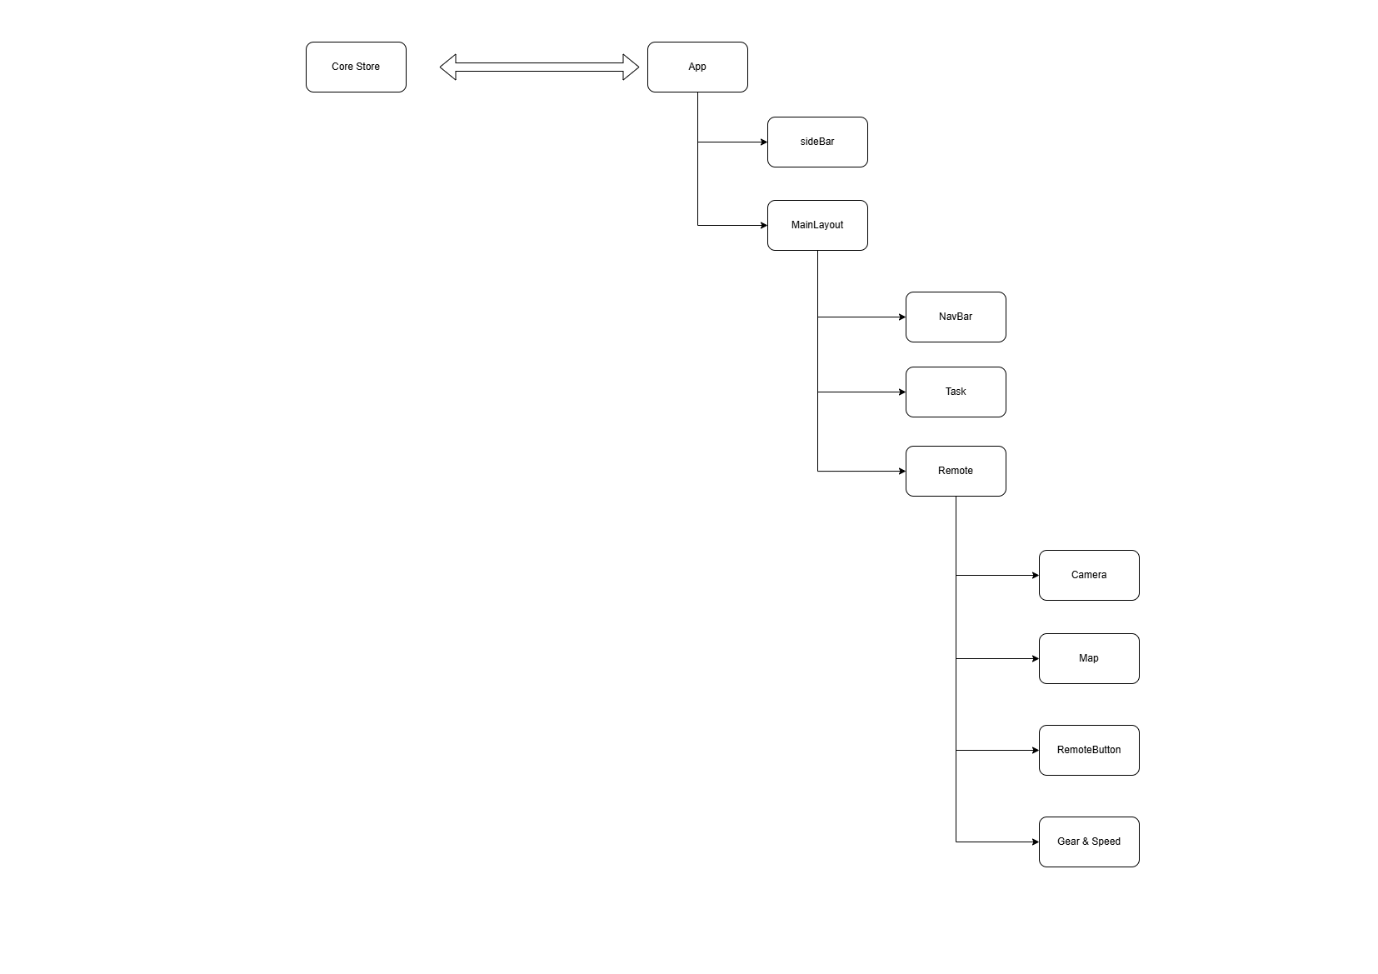
\includegraphics[width=6.26806in,height=4.42986in]{img/image001.png}
    \caption{GUI hierarchy}
    \label{judFig1}
    \end{figure}
    
    \subsection{Output}
    The graphical user interface of the robot, segmented into several
    functional areas for ease of operation:
    
    \begin{enumerate}
    \def\labelenumi{\arabic{enumi}.}
    \item
      \emph{Menu}: On the left side, we have a straightforward menu with two
      options: "Remote Control" and "Task." This menu allows users to
      navigate between different functionalities of the system easily (see
      \cref{judFig2}).
    \item
      \emph{Remote Control Tab}: This section is the heart of the interface
      and is further divided into three parts (see \cref{judFig3}):
    
      \begin{itemize}
      \item
        \emph{Main Camera View}: Dominating the top centre is a large grey
        box labelled "Main Camera." This is likely where the live feed from
        the camera appears, giving users a visual of the controlled
        environment.
      \item
        \emph{Control Panel}: Located below the camera view, this panel
        includes directional buttons (\emph{up, down, left, right}) and a
        central button labelled "S" for emergency stop
        There\textquotesingle s also a toggle switch marked "A" and "M" and
        a speed indicator displaying "0.00 m/s." These controls are probably
        used to manoeuvre the remote vehicle or robot.
      \item
        \emph{Map}: On the right side, we see a white area with a grid of
        blue squares, a red and green marker, likely indicating the position
        of the robot or points of interest. There are two additional buttons
        at the bottom, a blue one with a "+" sign and a red one with a "-"
        sign, possibly for zooming in and out.
      \end{itemize}
    \end{enumerate}
    
    \begin{figure}
    \centering
    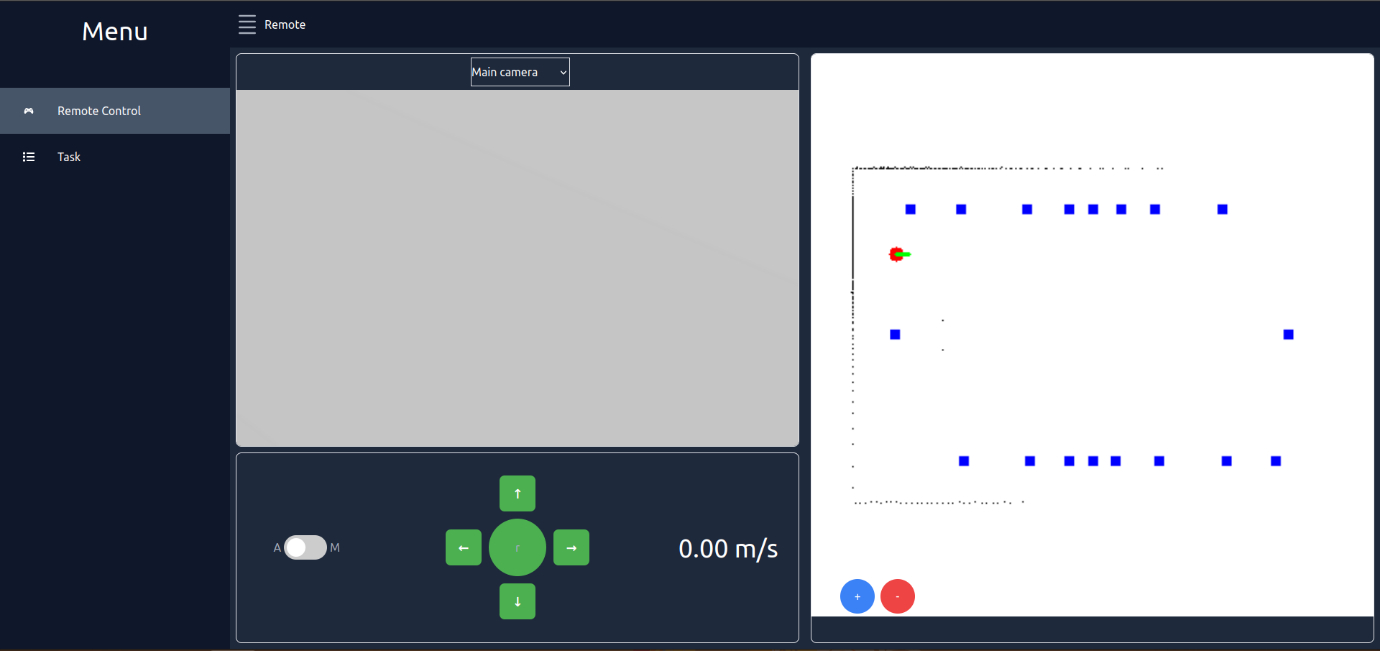
\includegraphics[width=6.26806in,height=2.95417in]{img/image003.png}
    \caption{Opened menu \& remote control Tab}
    \label{judFig2}
    \end{figure}
    
    \begin{figure}
    \centering
    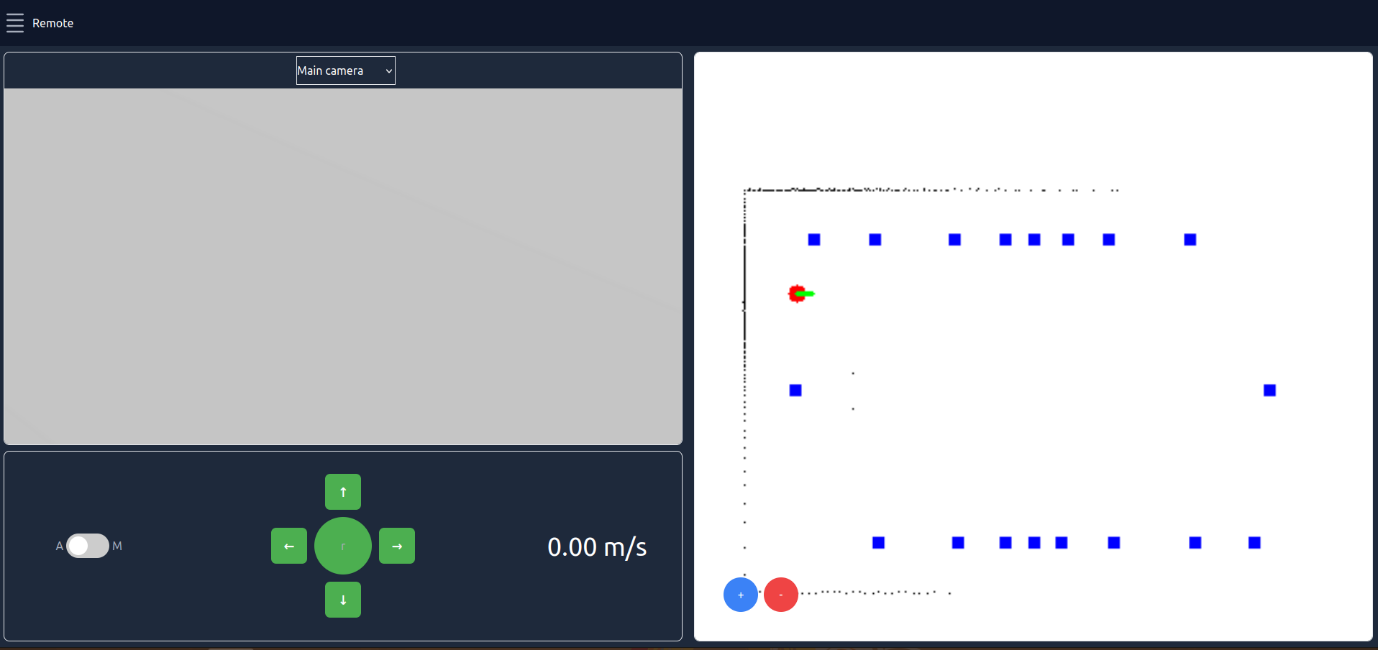
\includegraphics[width=6.26806in,height=2.95694in]{img/image005.png}
    \caption{Remote control tab}
    \label{judFig3}
    \end{figure}
    
    \begin{enumerate}
    \def\labelenumi{\arabic{enumi}.}
    \setcounter{enumi}{2}
    \item
      Task Tab: designed to manage tasks and monitor activities. The
      interface is divided into distinct sections for better functionality
      (\cref{judFig4}):
    
      \begin{itemize}
      \item
        \emph{Mapping Button}: This button is used to send the mapping task
        to the robot.
      \item
        \emph{Task Display}: Under the "Mapping" section,
        there\textquotesingle s a white text box labelled "Task display,"
        which displays tasks and other relevant information.
      \item
        \emph{Main Display Area}: The majority of the screen is occupied by
        a large dark area that serves as the main display or workspace for
        the system\textquotesingle s operations.
      \item
        \emph{Send Task Button}: At the bottom of the screen, this button
        allows users to send tasks to the robot.
      \end{itemize}
    \end{enumerate}
    
    This interface offers a clear, user-friendly design for effectively
    managing the robot.
    
    \begin{figure}[h!]
    \centering
    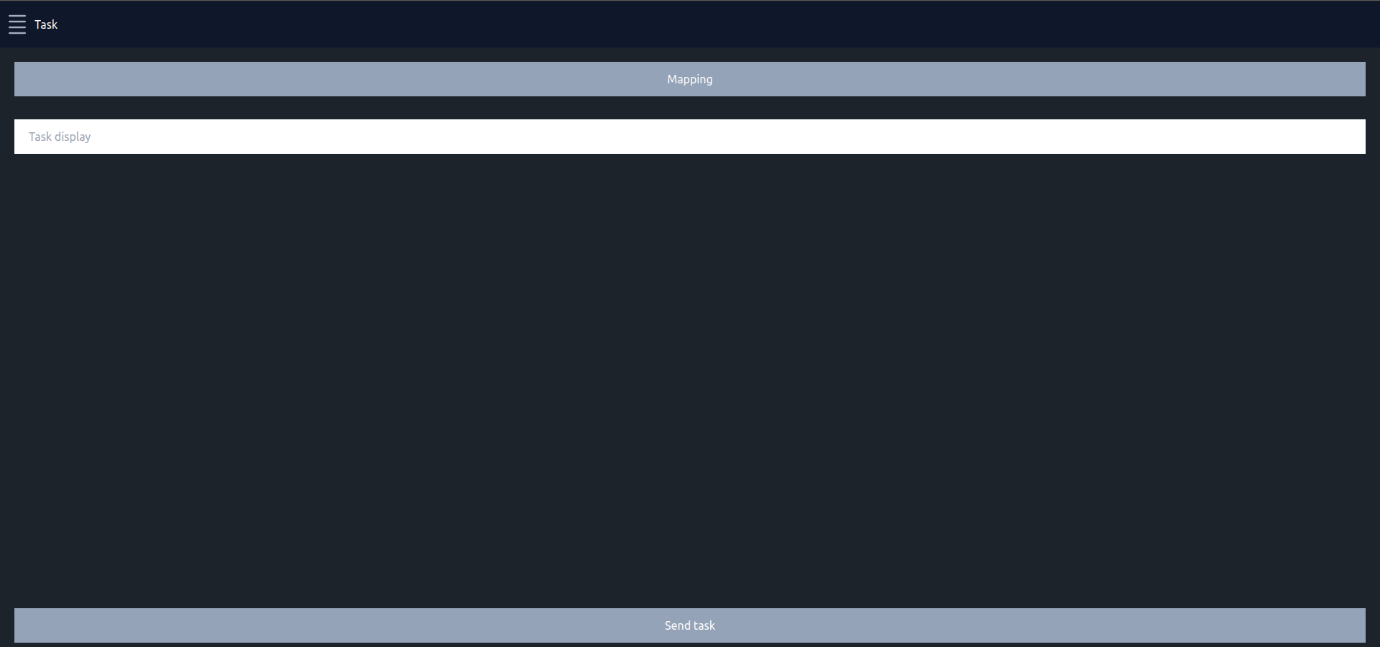
\includegraphics[width=6.26806in,height=2.93819in]{img/image007.png}
    \caption{Task Tab before mapping}
    \label{judFig4}
    \end{figure}
    
    \subsection{Codes and background implementation}
    
    \subsubsection{Core Store Implementation -- The Most Important Element}

    a centralized state management system using \emph{Zustand} to handle
application state, WebSocket communication, and real-time data updates.

\emph{Key Responsibilities and Implementation Details:}

State management was handled using \emph{Zustand} by creating a global
store (core, see \cref{judFig1}) to manage the application\textquotesingle s
state efficiently. This included tracking the connection status through
\emph{connectedSocket} and \emph{connectedRos}, as well as managing the
UI state with menu and \emph{menuOpened}. Real-time data, such as
\emph{cameraData}, \emph{camera\_qr\_data, mapData, speed, gear, zone,}
and \emph{station}, was also stored to ensure seamless updates.
Additionally, the application\textquotesingle s process state was
maintained using \emph{processState}. To facilitate state updates,
setter functions like \emph{setmenu} and \emph{setmenuOpened} were
implemented, allowing for specific property modifications.
\begin{figure}[h!]
\begin{minted}{js}
export const core = create((set,get) => 
({ connectedSocket : false,
    connectedRos : false,
    menu : "Remote",
    menuOpened : false,
    socket : null,
    cameraData : null,
    camera_qr_data : null,
    speed : 0,
    mapData : null,
    gear : 0,
    zone : null,
    station : null,}))

\end{minted}
\caption{All states of core element with their default value}
\end{figure}
\emph{WebSocket} integration was implemented using Socket.IO to enable
real-time communication between the frontend and backend. The
\emph{initializeSocket} function was developed to establish a connection
with the WebSocket server at \url{http://localhost:5000} (see \cref{judFig2}).
It managed connection and disconnection events, ensuring the
\emph{connectedSocket} state was updated accordingly. Additionally, it
listened for real-time data streams, including \emph{camera\_feed,
camera\_qr\_feed, map\_feed, speed, gear\_state, task\_response,
mapping\_output,} and \emph{processState}, allowing for seamless data
exchange and synchronization across the application.
\begin{figure}[h!]
  \begin{minted}{js}
  const socket = io('http://localhost:5000');
  set({ socket });
\end{minted}
\caption{socket connection}
\end{figure}


Real-time data handling was implemented to ensure seamless updates and
synchronization across the application. Camera feeds were processed and
stored as base64-encoded images in the state variables \emph{cameraData}
and \emph{camera\_qr\_data}, enabling real-time visualization. The
\emph{mapData} state was continuously updated with real-time map images
received from the backend. Additionally, the robot's speed and gear
state were tracked through WebSocket events, updating the speed and gear
properties accordingly. Task responses from the backend were displayed
using react-hot-toast, providing instant user feedback and enhancing the
overall user experience.

\begin{figure}
  \begin{minted}{js}
camera_feed : async function(data){
        set({cameraData : data.image})
    },
    camera_qr_feed : async function(data){
        set({camera_qr_data : data.image})
    },
    map_feed : async function(data){
        set({mapData : data.image})
    },
\end{minted}
\caption{socket connection}
\end{figure}
he frontend and backend. The \emph{sendTask} function was
implemented to transmit task sequences, such as loading and unloading,
to the backend via WebSocket. Task data, including \emph{task\_name} and
params, was structured and emitted through the \emph{robot\_task} event.
For mapping, the mapping function was triggered to initiate the process
by emitting a \emph{robot\_task} event with the necessary task data.
Additionally, the \emph{mapping\_output} event was processed to
serialize and store zone and station data in the state variables zone
and station, ensuring efficient real-time updates.

Serialization of mapping data was handled through the serialize function
(see \cref{judFig4}), which processed raw location data received from the
backend. This function filtered and organized intersection and station
data into structured formats, ensuring clarity and usability. The
processed data was then stored in the state variables zone and station,
enabling seamless integration with the UI for real-time visualization
and interaction.

\begin{figure}[h!]
  \begin{minted}{js}
serialize : async function(locations){
      let lcs = [], st = []
      locations.forEach(location => {
        let nm = location.location.split("_")
        if(nm[0] == "intersection"){
          if (nm[2] == "x" || nm[2] == "y"){ 
          }else{
            let found = false
            for(let i = 0; i < lcs.length; i++){
              if (lcs[i].location == nm[1] + " " + nm[2]){
                found = true
              }
            }
            if (!found){
              lcs.push({
                location : nm[1] + " " + nm[2],
                x : location.x, y : location.y,
              })
            }
          }
        }else if (nm[0] == "station"){
          let found = false
            for(let i = 0; i < st.length; i++){
              if (st[i].location == nm[0] + " " + nm[1]){
                found = true
              }
            }
            if (!found){
              st.push({location : nm[0] + " " + nm[1],
              x : location.x, y : location.y,
            })
          }
        }
      });
      set({zone : lcs})
      set({station : st})
    },
\end{minted}

\end{figure}
\newpage
Gear control was managed through the \emph{changeGear} function,
allowing the robot's gear state to toggle between \emph{automatic} and
\emph{manual} modes. To ensure safe operation, gear changes were
restricted while an active process was running \emph{(processState ===
"Processing")}. Additionally, react-hot-toast was used to provide user
feedback, notifying users when gear changes were blocked due to ongoing
tasks.

Direction control was handled through the \emph{sendDirection} function,
which transmitted movement commands such as \emph{UP, DOWN, LEFT}, and
\emph{RIGHT} to the backend via WebSocket. To maintain system integrity,
movement commands were restricted during active processes
\emph{(processState === "Processing")}, preventing conflicts with
ongoing tasks. User feedback was provided to ensure clarity when
movement commands were blocked.

The outcome was the successful delivery of a scalable and efficient
state management system that seamlessly integrates with WebSocket
communication. This integration enabled real-time updates for critical
data, including camera feeds, map data, speed, and gear state,
significantly enhancing the application\textquotesingle s interactivity
and responsiveness. Additionally, the system provided a robust
foundation for task management, mapping, and robot control, ensuring a
smooth and intuitive user experience while maintaining high performance
and reliability.

\subsubsection{App Component}

the root App component serves as the entry point for the application.

The application was enhanced with several key integrations to improve
functionality and user experience. \emph{React Router (BrowserRouter)}
was integrated to enable client-side routing, allowing for seamless
navigation between pages. Conditional rendering logic was added to
display a loading spinner (Loader component) while waiting for the
socket connection to be established, ensuring users are informed during
the connection process. The layout was structured using flexbox for a
responsive design, dividing the interface into a SideBar and MainLayout
component for better organization. Additionally, React Hot Toast
(Toaster) was integrated to provide user notifications and feedback,
enhancing interactivity and responsiveness throughout the application.

\emph{The outcome}:

The creation of a scalable and modular application structure, designed
to support real-time communication capabilities seamlessly. By
implementing loading states and real-time notifications, the application
ensures a smooth user experience, keeping users informed and engaged
during the connection process and throughout their interactions with the
system. This structure not only enhances performance but also improves
the overall user interface, making it responsive and intuitive. See
\cref{judFig9} for implementation.

\begin{figure}[h!]
  \begin{minted}{js}
function App() {
  const {initializeSocket, connectedSocket, connectedRos}= core()
  useEffect(function(){
    initializeSocket()
  },[initializeSocket])

  if(!(connectedSocket  )){
    return <Loarder/>
  }

  return (
    <BrowserRouter>
    <div className="flex flex-row w-full h-full">
        <SideBar />
        <MainLayout />
    </div>
    <Toaster></Toaster>
    </BrowserRouter>
  );
}

export default App;

\end{minted}
\caption{App Component}
\label{judFig9}
\end{figure}

\subsubsection{MainLayout Component}

This component manages the main content area and routing logic. See
\cref{judFig10} for implementation.

\emph{Key Responsibilities:}

The application was structured with React Router using Routes and Route
to define navigation paths. A default route (/) was set to render the
Remote component, while additional routes were configured for the
/remote path to display the Remote component and the /task path for the
Task component. Conditional rendering was implemented to display a
loading spinner (Loader component) when the socket connection is not yet
established, ensuring a smooth user experience during the initial
connection phase. The layout was designed to be responsive using CSS,
allowing the content area to adjust dynamically based on the viewport
size. Additionally, a \emph{NavBar} component was integrated at the top
of the layout to provide consistent navigation across the application,
enhancing usability and accessibility.

\emph{Outcome:}

Was the creation of a centralized and reusable layout structure for the
application, promoting maintainability and scalability. By implementing
proper loading states and routing, seamless navigation was ensured,
allowing users to transition between different sections smoothly. This
structure enhanced the overall user experience, providing consistent and
responsive design elements across the application, while also ensuring
that users are kept informed during the socket connection process.

\begin{figure}
\begin{minted}{js}
const MainLayout = () => {
    const { connectedSocket, menuOpened } = core();
    return (
    <div className="w-full h-full overflow-hidden">
        <NavBar />
        <div className="w-full h-[calc(100%-64px)]">
        <Routes>
            <Route path="/" element={connectedSocket ? <Remote /> : <Loader />} />
            <Route
            path="/remote"
            element={connectedSocket ? <Remote /> : <Loader />}
            />
            <Route path="/task" element={connectedSocket ? <Task /> : <Loader />} />
        </Routes>
        </div>
    </div>
    );
};
export default MainLayout;
\end{minted}
\caption{MainLayout Component}
\label{judFig10}
\end{figure}

\subsubsection{Remote Component}

Remote component serves as the central interface for remote control
functionality.

The application features a dual-panel layout implemented using \emph{CSS
Flexbox}, enhancing responsiveness and user experience. The left panel
integrates a live camera feed alongside a control interface equipped
with directional buttons (\emph{RemoteButton}) for navigation. A
gear-switching mechanism is incorporated, utilizing a toggle switch to
alternate between \emph{automatic (A)} and \emph{manual (M)} modes. This
functionality leverages \emph{React\textquotesingle s useEffect} and
\emph{useRef} \emph{hooks} for efficient state management. Throughout,
responsive and dynamic UI updates are ensured, adapting seamlessly to
user interactions and state changes. See code below for implementation.


  \begin{minted}{js}
const Remote = (props) => {
    const {sendDirection, changeGear, gear} = core()
    const gearref = React.createRef()
    const onReset = function(e){ sendDirection("STOP") }
    const switchGear = function(e){
        e.preventDefault()
        changeGear()
    }
    useEffect(() => { gearref.current.checked = gear == 1}, [gear])
return (
<div className="w-full h-full overflow-hidden flex flex-row bg-slate-800">
  <section className="w-1/2 p-2">
    <div className="w-full h-2/3 flex flex-col items-center  
    border rounded-lg overflow-hidden">
      <Camera/>
    </div>
    <div className="w-full h-[calc((100%/3)-8px)] 
    border rounded-lg mt-2 flex flex-row">
      <div className=" w-1/4 h-full flex items-center justify-center">
        <label className="switch-label mr-1">A</label>
          <label className="switch">
            <input type="checkbox" name="switch" 
            id = "switch" ref={gearref} value={gear == 1} onClick={switchGear}/>
              <span className="slider round"></span>
          </label>
        <label className="switch-label ml-1">M</label>
      </div>
      <div className="circle-section flex items-center justify-center  w-2/4 h-full">
        <div className="circle-container relative ">
          <button className="center-circle" onClick = {onReset}>r</button>
            <RemoteButton direction="UP"/>
            <RemoteButton direction="DOWN"/>
            <RemoteButton direction="LEFT"/>
            <RemoteButton direction="RIGHT"/>
        </div>
      </div>
      <div className=" w-1/4 h-full"><Speed/></div>
    </div>
  </section>
  <section className="w-1/2 flex items-center justify-center p-2">
    <div  className="w-full h-full border rounded-lg flex flex-col 
    items-center relative overflow-hidden">
      <Map ></Map>
    </div>
            </section>
    </div>
    );
};
export default Remote;
\end{minted}


\subsubsection{Camera Component}

The Camera component displays live camera feeds and enable camera
switching functionality.

A dynamic camera feed display was implemented by processing
base64-encoded image data from the backend, supporting both the Main
Camera and QR Code Camera. \emph{React\textquotesingle s useEffect} was
utilized to ensure the image source (\emph{imgRef}) updated whenever new
camera data (\emph{cameraData} or \emph{camera\_qr\_data}) was received
(see \cref{judFig12}). A camera selection dropdown was added to enhance user
interaction, allowing users to switch between the main camera and QR
code camera views. Memory management was efficiently handled by revoking
object URLs when the component unmounted or the camera data changed. The
component was styled using CSS to ensure the camera feed was responsive
and fit seamlessly within the layout.

\begin{figure}
  \begin{minted}{js}
useEffect(function(){
        if(cam === "front"){
            if (cameraData) {
                const imageUrl = `data:image/png;base64,${cameraData}`
                imgRef.current.src = imageUrl;

                // Clean up the object URL when component is unmounted
                return () => {
                    URL.revokeObjectURL(imageUrl);
                };
            }
        }
        else if (cam === "back"){
            if (camera_qr_data) {
                const imageUrl = `data:image/png;base64,${camera_qr_data}`
                imgRef.current.src = imageUrl;

                // Clean up the object URL when component is unmounted
                return () => {
                    URL.revokeObjectURL(imageUrl);
                };
            }
        }
    },[cameraData, camera_qr_data])
  \end{minted}
\caption{UseEffect which update camera image each render}
\label{judFig12}
\end{figure}
\newpage
\subsubsection{Map Component}

This component displays and interact with a dynamic map interface.
included integrating a base64-encoded map image (\emph{mapData}) to
display real-time map data. Zoom functionality was implemented using
buttons for zooming in (+) and out (-) (see code below), as well as mouse
wheel support for smooth zooming. A loading state was added to display a
placeholder message while the map data was being fetched. Using
\emph{useEffect}, the map image was dynamically updated whenever new
\emph{mapData} was received ( see code below), ensuring real-time
updates. CSS transformations (scale) were applied to enable smooth
zooming transitions, and floating zoom buttons were designed for an
intuitive user experience, styled with CSS for a modern look.


  \begin{minted}{js}
  const zoomIn = () => {
        setZoom((prevZoom) => Math.min(prevZoom + 0.1, 7)); // Max zoom 7x
    };

    const zoomOut = () => {
        setZoom((prevZoom) => Math.max(prevZoom - 0.1, 1)); // Min zoom 1x (original size)
    };

    const handleWheel = (event) => {
        // Prevent the page from scrolling when zooming
        event.preventDefault();
        
        if (event.deltaY < 0) {
            zoomIn(); // Zoom in when scrolling up
        } else {
            zoomOut(); // Zoom out when scrolling down
        }
    };

    useEffect(() => {
        if (mapData) {
            const imageUrl = `data:image/png;base64,${mapData}`;

            // Set image src only if imgRef.current is available
            imgRef.current.src = imageUrl;
            if(!mapData){
                setLoading(true);
            }
            setLoading(false)
            return () => {
                URL.revokeObjectURL(imageUrl);
            };
        }
    }, [mapData]);

\end{minted}



\subsubsection{Task Component}

the Task component manages task creation and submission for the
application. It is responsible for managing task creation and submission
for the application. The responsibilities included designing and
implementing a task creation interface that allowed users to select
zones and define tasks, such as loading or unloading. The component
dynamically built and displayed task sequences based on user input and
integrated validation logic (see code below) to ensure task sequences
adhered to predefined rules. For example, it prevented invalid task
combinations like unloading without loading first and limited the number
of tasks to a maximum of six. React hooks (\emph{useState, useEffect,
useCallback, useRef}) were utilized for state management and user
interaction handling. Toast notifications (react-hot-toast) were
integrated to provide real-time feedback for errors and successful
actions. A mapping button was implemented to trigger mapping
functionality and dynamically display available zones. The component was
styled using CSS and Tailwind CSS to achieve a clean and responsive
design, ensuring a smooth and intuitive user experience while
efficiently managing tasks within the application.

\begin{minted}{js}
const set = () => {
        if (params.length === 6) return toast.error("You can't load and unload more than 6 times");
        if (selected === "") return toast.error("Select a zone");
        let type = ref.current.value === "Loading" ? "L" : "U";
        if (type === "U") {
            let param = params[params.length - 1];
            if (param) {
                let key = Object.keys(param)[0];
                if (param[key] !== "Loading") {
                    return toast.error("You can't unload without loading");
                } else if (key === selected) {
                    return toast.error("You can't unload from a zone you've loaded from");
                }
            } else { return toast.error("You need to load first");}
        }else if( type === "L"){
            let param = params[params.length - 1];
            if (param) {
                let key = Object.keys(param)[0];
                if (param[key] === "Loading") {
                    return toast.error("You can't load twice");
                }
            }
        }
        setTask(`${task}${selected}(${type}) -> `);
        setParams([...params, { [selected]: ref.current.value }]);
        setSelected("");
    };
\end{minted}



\section{ROS}
The Robot Operating System (ROS) serves as the robot\textquotesingle s
main controller, managing all operations seamlessly at all times and
facilitating communication with the GUI.

\begin{figure}[h!]
\centering
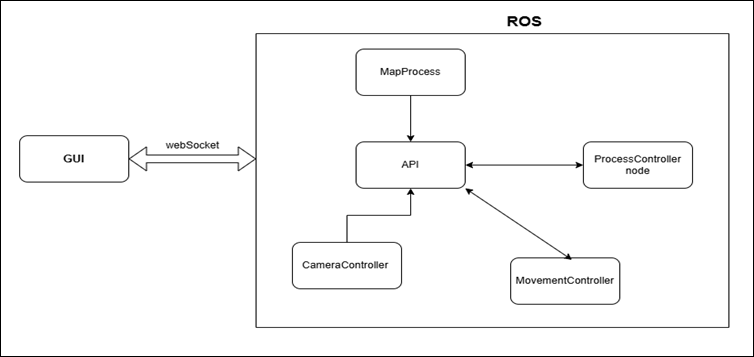
\includegraphics[width=\textwidth]{img/image022.png}
\caption{general architecture}
\label{judFig15}
\end{figure}

\begin{figure}[h!]
\centering
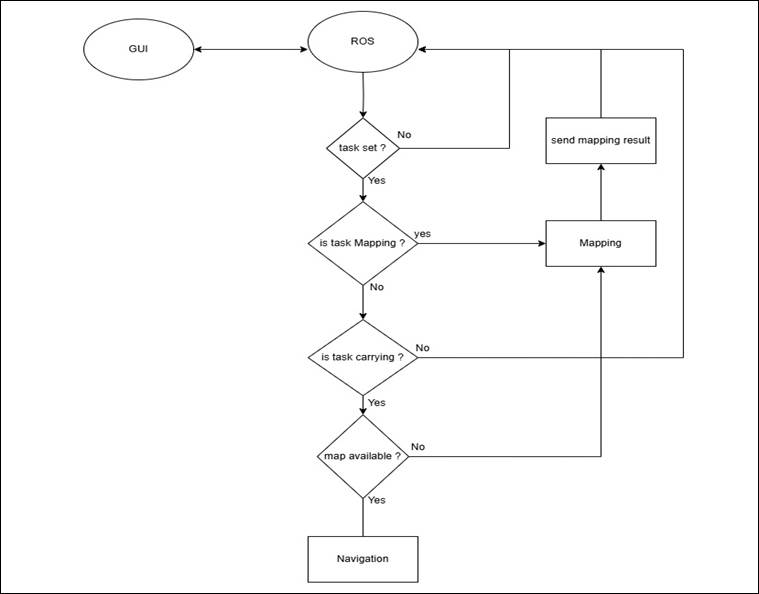
\includegraphics[width=\textwidth]{img/image024.jpg}
\caption{general architecture}
\end{figure}

\subsection{Nodes}

\subsubsection{ie\_API\_Server}

This node serves as a critical bridge between the ROS (Robot Operating
System) ecosystem and a frontend application, leveraging
\emph{WebSocket} communication to enable seamless interaction. It
facilitates real-time data streaming, robot control, and task
management, ensuring smooth and efficient communication between the
backend and frontend (see \cref{judFig15}).

\begin{figure}[h!]
  \begin{minted}{python}
  class ie_API_Server:
    def __init__(self):
        self._bridge = CvBridge()
        self.sio = socketio.async_server.AsyncServer(async_mode='asgi', cors_allowed_origins="*")
        self.app = socketio.asgi.ASGIApp(self.sio)
        self.mc_pub = rospy.Publisher("manual_controller", Int32, queue_size=10)
        self.cam_sub = rospy.Subscriber("camera_feed", Image, self.run_async_cameraFeedCallback)
        self.cam_qr_sub = rospy.Subscriber("camera_qr_code_feed", Image, self.run_async_cameraQrFeedCallback)
        self.sensors_sub = rospy.Subscriber("sensor_data", SensorDataMap, self.sensorsCallback)
        self.speed_sub = rospy.Subscriber("speed_value", Float32, self.run_async_speedCallback)
        self.map_sub = rospy.Subscriber("map_feed", Image, self.run_async_mapFeedCallback)
        self.process_sub = rospy.Subscriber("ProcessState", String, self.run_async_processState)
        rospy.Service('output', taskMessage, self.run_async_taskFinished)
        rospy.Service('mapping_output', mappingOutput, self.run_async_mappingOutput)
        rospy.Service('gear_changed', robotGear, self.run_async_gearChanged)
        self.sio.on("connect", self.onConnect)
        self.sio.on("disconnect", self.onDisconnect)
        self.sio.on("moveDirection", self.movement)
        self.sio.on("message", self.message)
        self.sio.on("robot_task", self.taskCallback)
        self.sio.on("robot_gear", self.gearCallback)
\end{minted}
\caption{API initial value}
\label{judFig16}
\end{figure}

The node integrates~\emph{WebSocket
communication}~using~\emph{Socket.IO}, establishing a real-time,
bidirectional channel that supports multiple clients. This allows users
to connect, disconnect, and interact with the robot in real time. The
WebSocket connection is the backbone of the system, enabling instant
data exchange and control commands between the frontend and the ROS
backend.
\newpage
\begin{figure}[h!]
  \begin{minted}{python}
  # Register event handlers
self.sio.on("connect", self.onConnect)
self.sio.on("disconnect", self.onDisconnect)
self.sio.on("moveDirection", self.movement)
self.sio.on("message", self.message)
self.sio.on("robot_task", self.taskCallback)
self.sio.on("robot_gear", self.gearCallback)
\end{minted}
\caption{API initial value}
\label{judFig17}
\end{figure}

For~\emph{real-time data streaming}, the node subscribes to various ROS
topics to capture and process critical information. It subscribes
to~\emph{camera\_feed}~and~\emph{camera\_qr\_code\_feed}~to receive live
camera images, which are then converted from ROS Image messages to
OpenCV format using~\emph{CvBridge}. These images are encoded
as~\emph{base64 strings}~and streamed to the frontend via WebSocket.
Similarly, the node subscribes to the~\emph{map\_feed}~topic to receive
real-time map images, processes them, and streams them to the frontend
in the same manner. Additionally, it subscribes to
the~\emph{speed\_value}~topic to capture the robot's speed and emits
speed updates to the frontend in real time, ensuring users have
up-to-date information on the robot's movement.

The node also handles~\emph{robot control}~by listening for specific
events from the frontend. For movement control, it listens
for~\emph{moveDirection}~events (e.g., \emph{UP, DOWN, LEFT, RIGHT,
STOP}) and translates these into corresponding commands published to
the~\emph{manual\_controller} ROS topic, enabling direct control of the
robot's movement. For gear control, it listens
for~\emph{robot\_gear}~events to toggle between automatic and manual
modes. This is achieved by calling the~\emph{change\_gear}~ROS service
and emitting the updated gear state to the frontend, ensuring the user
interface reflects the current state of the robot.

\emph{Task management}~is another key functionality of the node. It
listens for~\emph{robot\_task}~events from the frontend, which trigger
tasks such as loading, unloading, or mapping. The node converts task
data into a ROS-compatible format (using the~\emph{TaskData}~message)
and calls the~\emph{robot\_task}~service to execute the task(see \cref{judFig17}). It also listens for task feedback from the ROS backend via
the~\emph{output}~service, emitting task responses (e.g., success or
failure messages) to the frontend. This ensures users receive timely
updates on task progress and outcomes, enhancing transparency and
usability.

For~\emph{mapping functionality}, the node listens for mapping data from
the ROS backend via the~\emph{mapping\_output}~service. It processes and
serializes this data, which includes information such as locations and
coordinates, and emits it to the frontend. This allows users to
visualize the robot's environment and track its movements in real time.

Finally, the node monitors the robot's~\emph{process state}~by
subscribing to the~\emph{ProcessState}~topic. It captures updates on the
robot's current state (e.g., Processing, Stationary) and emits these
updates to the frontend in real time. This ensures users are always
aware of the robot's operational status, enabling better decision-making
and control.


  \begin{minted}{python}
  async def taskCallback(self, sid, task):
        t = TaskData()
        t.task_name = task['task']["task_name"]
        t.params =  [Param(zone=key,type=value) for key, value in task['task']["params"].items()]
        rospy.wait_for_service('robot_task')
        robot_task = rospy.ServiceProxy('robot_task', robotTask)
        robot_task.wait_for_service(10)
        try:
            response = robot_task(t)
            print(response)
            await self.sio.emit("task_response", {"response": response.message}, to=sid)
        except rospy.ServiceException as exc:
            print("Service did not process request: " + str(exc))   

    def run_async_taskFinished(self,output):
        try:
            loop = asyncio.new_event_loop()
            asyncio.set_event_loop(loop)
            loop.run_until_complete(self.taskFinished(output))
        except Exception as e:
            rospy.logerr(f"Error before proccessing and emitting taskFinished: {e}")

        return taskMessageResponse(True)
    
    async def taskFinished(self, output):
        await self.sio.emit("task_response", {"response": output.message})

    def run_async_mappingOutput(self,output):
        try:
            loop = asyncio.new_event_loop()
            asyncio.set_event_loop(loop)
            loop.run_until_complete(self.mappingOutput(output))
        except Exception as e:
            rospy.logerr(f"Error before proccessing and emitting taskFinished: {e}")

        return mappingOutputResponse(True)
    
    async def mappingOutput(self, output):
        print(output)
        data = [{"location" :kv.location, "x": kv.x, "y":kv.y} for kv in output.locations]
        print(data)
        await self.sio.emit("mapping_output", {"locations": data})
\end{minted}


\subsubsection{movementController}

This node manages the robot's movement in both \emph{manual} and
\emph{autonomous} modes. It processes control commands, handles gear
switching, and ensures smooth transitions between states.

\emph{Key Features and Functionality}:

The node supports two modes of operation:

\begin{itemize}
\item
  \emph{Manual Mode}: The robot is controlled via user commands, such as
  increasing or decreasing linear or angular velocity.
\item
  \emph{Autonomous Mode}: The robot is controlled by an external system,
  like a navigation stack, with manual control disabled.
\end{itemize}

To facilitate seamless switching between these modes, the
\emph{twist\_mux} package can be utilized. This package subscribes to
multiple \emph{cmd\_vel} topics.

The Movement Control component was designed to subscribe to the
\emph{manual\_controller} topic to receive movement commands, such as
\emph{UP, DOWN, LEFT, RIGHT,} and \emph{STOP}. The component adjusted
the robot\textquotesingle s linear and angular velocity based on the
received commands and then published the resulting velocity commands to
the \emph{cmd\_vel} topic.

Gear Switching system provides a ROS service (\emph{change\_gear}) to
switch between manual and autonomous modes, updates the gear state and
notifies the GUI via another ROS service (\emph{gear\_changed}) (see
\cref{judFig15}). Velocity Interpolation Implements smooth interpolation for
angular velocity to prevent abrupt changes in robot movement. Uses a
waiting period and linear interpolation to gradually reduce angular
velocity to zero.

Process State Monitoring Subscribes to the \emph{ProcessState} topic to
monitor the robot's current state (e.g., Processing, Stationary). Resets
movement commands if the robot is in a Processing state. Speed
Calculation Calculates the robot's total velocity by combining linear
and angular velocity components. Publishes the calculated speed to the
\emph{speed\_value} topic for real-time monitoring.

\emph{Technical Details}:

\begin{itemize}
\item
  ROS Integration:

  \begin{itemize}
  \item
    Publishers:

    \begin{itemize}
    \item
      cmd\_vel: Publishes velocity commands for the robot.
    \item
      speed\_value: Publishes the robot's current speed.
    \end{itemize}
  \item
    Subscribers:

    \begin{itemize}
    \item
      manual\_controller: Receives movement commands.
    \item
      ProcessState: Monitors the robot's state.
    \item
      cmd\_vel: Receives velocity commands from the autonomous system.
    \end{itemize}
  \item
    Services:

    \begin{itemize}
    \item
      change\_gear: Handles gear switching between manual and autonomous
      modes.
    \end{itemize}
  \end{itemize}
\item
  Data Structures:

  \begin{itemize}
  \item
    cmd\_vel Struct: Stores the robot's linear and angular velocity (see
    \cref{judFig17}) components.Manages interpolation and waiting states for
    smooth velocity transitions.Provides methods to increase/decrease
    velocity and reset commands.
  \end{itemize}
\item
  Interpolation Logic: Uses timestamps (ros::Time) to track the last
  update time and interpolation duration. Implements a waiting period
  (wait\_duration) before starting interpolation. Linearly interpolates
  angular velocity towards zero over a specified duration
  (interpolation\_duration), see \cref{judFig16} for implementation.
\item
  Velocity Calculation: Combines linear and angular velocity components
  to calculate the robot's total velocity. Accounts for the robot's
  wheel radius (radius) to convert angular velocity to linear velocity.
\item
  Error Handling: Logs warnings for invalid commands or attempts to
  control the robot in autonomous mode. Ensures smooth transitions
  between states to prevent abrupt movements.
\end{itemize}

\begin{figure}
  \begin{minted}{cpp}
  bool changeGear (ie_communication::robotGear::Request &req, ie_communication::robotGear::Response &res){
    movedata.gear = req.state;
    if(movedata.gear == 0){
        std::cout << "The robot is in autonomous mode, manual control is disabled" << std::endl;
    }else{
        std::cout << "The robot is in manual mode, autonomous control is disabled" << std::endl;
    }

    ros::NodeHandle n;
    ros::ServiceClient client = n.serviceClient<ie_communication::robotGear>("gear_changed");
    ie_communication::robotGear srv;

    srv.request.state = movedata.gear;

    if(client.call(srv)){

    }else{
        ROS_ERROR("Failed to update the gear to GUI");
    }

    res.message = true;
    return true;
}
\end{minted}
\caption{Gear shift}
\end{figure}

\begin{figure}
  \begin{minted}{cpp}
  void updateAngular() {
        ros::Time current_time = ros::Time::now();
        ros::Duration time_since_update = current_time - last_update_time;

        if (waiting_to_interpolate) {
            if (time_since_update.toSec() >= wait_duration) {
                // Start interpolation after waiting period
                angular_start = az;
                interpolation_start_time = current_time;
                angular_interpolating = true;
                waiting_to_interpolate = false;
            }
        }

        if (angular_interpolating) {
            ros::Duration time_since_start = current_time - interpolation_start_time;
            float t = time_since_start.toSec() / interpolation_duration;

            if (t >= 1.0) {
                az = 0.0; // Stop interpolation after duration
                angular_interpolating = false;
            } else {
                az = angular_start * (1.0 - t); // Linearly interpolate towards zero
            }
        }
    }

\end{minted}
\caption{Linear interpolation}
\end{figure}


  \begin{minted}{cpp}
  struct cmd_vel {
    int gear = 0;
    float lx = 0.0;
    float ly = 0.0;
    float lz = 0.0;
    float ax = 0.0;
    float ay = 0.0;
    float az = 0.0;

    ros::Time last_update_time; // Last time angular velocity was updated
    ros::Time interpolation_start_time; // Time when interpolation starts
    bool angular_interpolating = false; // Flag to indicate interpolation
    bool waiting_to_interpolate = false; // Flag to indicate waiting period
    float angular_start = 0.0; // Starting value for interpolation
    float interpolation_duration = 0.8; // Duration for interpolation (in seconds)
    float wait_duration = 0.3; // Time to wait before starting interpolation (in seconds)
    float radius = 0.16;
    void changeGear(const std_msgs::Int32::ConstPtr& msg) {
        gear = msg->data;
    }
    void increaseLinear() {
        lx += 0.01;
    }

    void decreaseLinear() {
        lx -= 0.01;
    }

    void increaseAngular() {
        az += 0.1;
        updateAngularState();
    }

    void decreaseAngular() {
        az -= 0.1;
        updateAngularState();
    }

    void reset() {
        lx = 0.0;
        ly = 0.0;
        lz = 0.0;

        ax = 0.0;
        ay = 0.0;
        az = 0.0;

        angular_interpolating = false;
        waiting_to_interpolate = false;
    }

    void updateAngularState() {
        last_update_time = ros::Time::now();
        angular_interpolating = false; // Stop interpolation if active
        waiting_to_interpolate = true; // Set waiting state
    }

    
    float getVelocity(){
        if (gear == 1){
            float linear_velocity_rotational = az * radius;
            float tVelocity = sqrt((pow(lx, 2) + pow(linear_velocity_rotational, 2)));
            return std::round(tVelocity * 100.0f) / 100.0f;
        }else{
            float linear_velocity_rotational = acvl.angular.z * radius;
            float tVelocity = sqrt((pow(acvl.linear.x, 2) + pow(linear_velocity_rotational, 2)));
            return std::round(tVelocity * 100.0f) / 100.0f;
        }
    }
};

\end{minted}
% \caption{Cmd\_vel structure}
\noindent
\captionof{figure}{Cmd\_vel structure}\label{judeFig21}




\subsubsection{CameraController}

This node functions as a~\emph{camera feed manager}, playing a crucial
role in subscribing to raw camera feeds, processing them, and publishing
the processed feeds to other ROS topics for further use, such as display
or analysis. It subscribes to two raw camera
feeds: \emph{/camera/rgb/image\_raw}, which is the primary camera feed
used for general purposes like navigation or object detection,
and~\emph{/camera\_2/camera\_2/image\_raw}, the secondary camera feed
often utilized for specialized tasks such as QR code detection. The node
then publishes the processed feeds to two ROS
topics:~\emph{camera\_feed}~for the primary camera feed
and~\emph{camera\_qr\_code\_feed}~for the secondary camera feed. This
ensures that downstream nodes or applications have access to the
necessary camera data for their respective tasks, see \cref{judeFig21} for
implementation.

The node also incorporates~\emph{camera state management}~to ensure
efficient operation. It uses a \emph{boolean flag (\_camState)} to
enable or disable feed publishing, ensuring that feeds are only
published when the camera is active and data is available. Additionally,
it tracks camera availability \emph{(\_cam\_available}) to prevent
publishing when no data is being received. This state management
mechanism helps optimize resource usage and prevents unnecessary
processing. To handle potential issues, the node implements~\emph{robust
error handling}~for image conversion and publishing. Errors, such as
failed image conversions or publishing failures, are logged
using~\emph{rospy.logerr}, making it easier to debug and maintain the
system.

From a technical perspective, the node integrates seamlessly with the
ROS ecosystem. It subscribes
to~\emph{/camera/rgb/image\_raw}~and~\emph{/camera\_2/camera\_2/image\_raw}~to
receive raw images from the primary and secondary cameras, respectively.
It then publishes the processed images
to~\emph{camera\_feed~}and\emph{~camera\_qr\_code\_feed}~for further
use. For image processing, the node uses~\emph{CvBridge}~to convert ROS
Image messages into OpenCV-compatible formats. While the node processes
and publishes the images, it does not apply additional filtering or
transformations, ensuring the images remain in their original state
unless modified by downstream nodes.

To ensure smooth operation and responsiveness, the node is initialized
in a~\emph{separate thread}. This threading approach allows the node to
handle image processing and publishing without blocking the main thread,
ensuring efficient performance even under high workloads. By combining
ROS integration, state management, error handling, and threading, this
camera feed manager node provides a reliable and efficient solution for
managing and streaming real-time camera data within the ROS ecosystem.
Its design ensures that downstream applications receive the necessary
camera feeds promptly and accurately, making it an essential component
for systems that rely on real-time visual data.


  \begin{minted}{python}
  import rospy
from ie_communication.srv import camState, camStateResponse
import cv2
from cv_bridge import CvBridge
from sensor_msgs.msg import Image

class CameraController:

    def __init__(self):
        self._pubcam1 = rospy.Publisher("camera_feed", Image, queue_size=10)
        self._pubcam2 = rospy.Publisher("camera_qr_code_feed", Image, queue_size=10)
        rospy.Subscriber("/camera/rgb/image_raw",Image, self._camera1Process)
        rospy.Subscriber("/camera_2/camera_2/image_raw",Image, self._camera2Process)
        self._bridge = CvBridge()
        self._camState = True
        self._cam_available = False
        self._cam1Frame = None
        self._cam2Frame = None

    def _camera1Process(self, data):
        try:
            self._cam1Frame = data
            self._cam_available = True
            self._provideCamFeed()
        except Exception as e:
            rospy.logerr(f"Error converting image: {e}")

    def _camera2Process(self, data):
        try:
            self._cam2Frame = data
            self._cam_available = True
            self._provideCam2Feed()
        except Exception as e:
            rospy.logerr(f"Error converting image: {e}")

    def _provideCamFeed(self) -> None:
        if self._camState and self._cam_available:
            try:
                self._pubcam1.publish(self._cam1Frame)
            except Exception as e:
                rospy.logerr(f"Error publishing image feed: {e}")

    def _provideCam2Feed(self) -> None:
        try:
            self._pubcam2.publish(self._cam2Frame)
        except Exception as e:
            rospy.logerr(f"Error publishing image from cam2 feed: {e}")
\end{minted}
% \caption{CameraProcess node}
\captionof{figure}{CameraProcess node}\label{judFig22}


\subsubsection{map\_process}

This node is responsible for processing laser scan data, robot position,
and QR code positions to generate and publish a dynamic map for
visualization and navigation. It subscribes to the~\emph{/scan}~topic to
receive laser scan data, which is processed to detect obstacles and
update the local map. The robot's position and orientation are tracked
using~\emph{TF2}, which retrieves the robot's translation and rotation
in the map frame. These coordinates are then converted into pixel
coordinates for visualization on the map. Additionally, the node
integrates QR code positions by reading them from an SQLite database
(\emph{qr\_code.db}) every 5 seconds. These QR code positions are
displayed on the map as blue rectangles, providing a comprehensive view
of the environment.

\begin{figure}
  \begin{minted}{python}
  def update_map_from_scan(self):
    if self.robot_position is None or self.robot_rotation is None:
       return
    yaw = self.get_yaw_from_quaternion(self.robot_rotation)

    for i, range_val in enumerate(self.latest_scan.ranges):
        if range_val < self.latest_scan.range_min or range_val > self.latest_scan.range_max:
            continue  # Skip invalid range values
            
  angle=self.latest_scan.angle_min+i* self.latest_scan.angle_increment

        endpoint_x = self.robot_position.x + range_val * np.cos(yaw + angle)
        endpoint_y = self.robot_position.y + range_val * np.sin(yaw + angle)

        endpoint_x_pixel = int((endpoint_x - self.map_origin_x) / self.map_resolution)

        endpoint_y_pixel = int((endpoint_y - self.map_origin_y) / self.map_resolution)
            
        if 0 <= endpoint_x_pixel < self.map_width and 0 <= endpoint_y_pixel < self.map_height:
                
                self.map_image[endpoint_y_pixel, endpoint_x_pixel] = 0

\end{minted}
\caption{Update Map from Scan Function}
\end{figure}

\newpage
The node generates a~\emph{2D map image}~that includes several key
elements: obstacles derived from laser scan data (represented as black
pixels), the robot's current position (shown as a red circle) and
orientation (indicated by a green line), QR code positions (displayed as
blue rectangles), and the robot's path (traced as a green line over
time). This map image is published to the~\emph{map\_feed}~topic,
enabling real-time visualization for users or other nodes. The map is
dynamically updated at a fixed rate of 10 Hz using a timer callback,
ensuring it reflects the latest scan data, robot position, and QR code
positions. The map parameters, such as resolution (5 cm per pixel),
dimensions (\emph{400x400 pixels}), and origin \emph{(-10.0, -10.0
meters}), are predefined, and the map is initialized as free space
(white pixels) before being updated with obstacles (black pixels) from
laser scans.

In summary, this node provides a dynamic and real-time map visualization
by integrating laser scan data, robot position, and QR code positions.
Its robust processing and integration capabilities ensure accurate and
up-to-date map generation, making it a vital component for navigation
and visualization tasks in the ROS ecosystem.


  \begin{minted}{js}
  def process_scan(self):
        self.map_image.fill(255)  

        robot_x_pixel = int((self.robot_position.x - self.map_origin_x) / self.map_resolution)
        robot_y_pixel = int((self.robot_position.y - self.map_origin_y) / self.map_resolution)

        if not (0 <= robot_x_pixel < self.map_width and 0 <= robot_y_pixel < self.map_height):
            return
      self.update_map_from_scan()
      map_image_color=cv2.cvtColor(self.map_image, cv2.COLOR_GRAY2BGR)

      if len(self.path_history) > 1:
          for i in range(1, len(self.path_history)):
                cv2.line(map_image_color, self.path_history[i - 1], self.path_history[i], (0, 255, 0), 2)

      for qr_x, qr_y in self.qr_code_positions:
          qr_x_pixel=int((qr_x-self.map_origin_x)/ self.map_resolution)
          qr_y_pixel=int((qr_y-self.map_origin_y)/ self.map_resolution)
            if 0 <= qr_x_pixel < self.map_width and 0 <= qr_y_pixel < self.map_height:
                cv2.rectangle(map_image_color,
(qr_x_pixel - self.qr_code_size, qr_y_pixel - self.qr_code_size),(qr_x_pixel + self.qr_code_size, qr_y_pixel + self.qr_code_size),(255, 0, 0), -1)

        cv2.circle(map_image_color, (robot_x_pixel, robot_y_pixel), 5, (0, 0, 255), -1)
        yaw = self.get_yaw_from_quaternion(self.robot_rotation)
        robot_x_end = robot_x_pixel + int(np.cos(yaw) * 10)
        robot_y_end = robot_y_pixel + int(np.sin(yaw) * 10)
        cv2.line(map_image_color, (robot_x_pixel, robot_y_pixel), (robot_x_end, robot_y_end), (0, 255, 0), 2)

        map_image_color = np.flipud(map_image_color)
        map_image_color = cv2.rotate(map_image_color, cv2.ROTATE_90_COUNTERCLOCKWISE)
        output_path = "/tmp/robot_map_with_position.png"
        cv2.imwrite(output_path, map_image_color)
        self.send_image(output_path)
\end{minted}
% \caption{Function Drawing Map}
\captionof{figure}{Function Drawing Map}\label{judeFig24}

\subsection{Classes}

\subsubsection{Task}

The Task class is a base class that encapsulates common functionality
for robot tasks, such as: Robot \emph{control} (movement, turning,
stopping), \emph{Obstacle detection and avoidance} \\using LIDAR data,
\emph{Image processing} for line following and QR code detection,
\emph{State management} for task execution and transitions.

\emph{Key Features and Functionality:}

The robot control system offers a comprehensive set of methods for
managing basic robot movements. These include \emph{\_move\_forward},
which propels the robot forward at a constant speed, as well \emph{as
\_turn\_left} and \emph{\_turn\_right} for executing left and right
turns, respectively. Additionally, the system features a
\emph{\_U\_turn} method for performing a 180° turn and a \emph{\_move}
function that adjusts the robot's movement based on error, particularly
useful for tasks like line following. To halt the robot, the \emph{stop}
method is available.

For obstacle detection and avoidance, the system subscribes to the
\emph{/scan} topic to receive LIDAR data, enabling it to monitor the
surroundings. It employs the \emph{check\_for\_obstacles} function (see
\cref{judFig22}) to detect obstacles in the robot's path. When an obstacle is
detected, the system utilizes a contouring algorithm called
\emph{contour\_obstacle(see} \cref{judFig22}\emph{)} to navigate around it.
This algorithm involves turning 90° left, moving forward, turning 90°
right, and then returning to the original path. To ensure precise turns,
the system tracks the robot's orientation using odometry data, accessed
through the \emph{\_get\_yaw} method. This combination of movement
control and obstacle avoidance ensures efficient and accurate navigation
in dynamic environments.

\begin{figure}[h!]
  \begin{minted}{python}
  def contour_obstacle(self):
        self._contourningStep += 1 
        if self.timer:
            self.timer.shutdown()  
        self.stop()  # Stop the robot
        
        if self._contourningStep == 1:
            rospy.loginfo("Contouring obstacle: Step 1")
            self.turn_angle(90)  
            self.contour_obstacle()
        elif self._contourningStep == 2:
            rospy.loginfo("Contouring obstacle: Step 2")
            self._move_forward()  
            while not self.is_obstacle_behind():
                rospy.sleep(0.1)
            self.turn_angle(-90)  # Turn right 90°
            self.contour_obstacle()
        elif self._contourningStep == 3:
            rospy.loginfo("Contouring obstacle: Step 3")
            self._move_forward()  
            while not self.is_obstacle_behind():
                rospy.sleep(0.1)
            self.turn_angle(-90)  
            self.contour_obstacle()
        elif self._contourningStep == 4:
            rospy.loginfo("Contouring obstacle: Step 4")
            self._move_forward()  
            self._turnSide = "left"
            self.moveToTurnPosition = True
            self._obstacleInFront = False
\end{minted}
\caption{Obstacle avoidance procedure}
\end{figure}
\begin{figure}[h!]
  \begin{minted}{python}
  def is_obstacle_behind(self):
        if self.scan_data is None:
            return False  
        robot_length = 0.52  
        obstacle_distance_threshold = robot_
        sector_start_angle = np.deg2rad(225)  # 225 degrees
        sector_end_angle = np.deg2rad(270)   # 270 degrees
        angle_increment = self.scan_data.angle_increment
        num_ranges = len(self.scan_data.ranges)
        start_index = int((sector_start_angle - self.scan_data.angle_min) / angle_increment)
        end_index = int((sector_end_angle - self.scan_data.angle_min) / angle_increment)
        min_distance = float('inf')
        for i in range(start_index, end_index):
            if 0 < self.scan_data.ranges[i] < min_distance:
                min_distance = self.scan_data.ranges[i]
        print(f"min distance : {min_distance}")
        return min_distance > obstacle_distance_threshold and min_distance < (obstacle_distance_threshold + 0.5)
\end{minted}
\caption{Function checking if the robot overpass the obstacle}
\end{figure}
\begin{minted}{python}
  def check_for_obstacles(self, event):
    if self.scan_data is None or len(self.scan_data.ranges) == 0:
      return  

print("Checking for obstacles using LIDAR data")
  front_angle_range = 30  # Degrees
    front_angle_range_rad = np.deg2rad(front_angle_range)
    angle_increment = self.scan_data.angle_increment
    num_ranges = len(self.scan_data.ranges)
    min_angle = self.scan_data.angle_min
    start_index = max(0, int((min_angle - front_angle_range_rad / 2) / angle_increment))
    end_index = min(num_ranges - 1, int((min_angle + front_angle_range_rad / 2) / angle_increment))
    min_distance = float('inf')
    for i in range(start_index, end_index):
      if 0 < self.scan_data.ranges[i] < min_distance and np.isfinite(self.scan_data.ranges[i]):
          min_distance = self.scan_data.ranges[i]
          obstacle_distance_threshold = 0.3  
    if min_distance < obstacle_distance_threshold:
        self._obstacleInFront = True
        rospy.loginfo(f"Obstacle detected at {min_distance:.2f} meters!")
        self.stop()  # Stop the robot
        self._obstacleChecker += 1

    if self._obstacleChecker >= 5:
      rospy.loginfo("Obstacle is still present. Calling contour_obstacle function.")
      self._obstacleChecker = 0

    if not self._contourningObstacle:
        self._contourningObstacle = True
        self.contour_obstacle()
    else:
        self._obstacleInFront = False
        self._obstacleChecker = 0  
        rospy.loginfo("No obstacle detected. Moving.")
\end{minted}
\captionof{figure}{Obstacle Detection}\label{judFig26}

\newpage
The image processing component of the system is designed to enhance the
robot\textquotesingle s navigation and interaction capabilities by
subscribing to multiple camera topics, such as\\
\emph{/camera/rgb/image\_raw} and \emph{/camera\_qr\_code\_feed}. This
allows the robot to perform tasks like line following and QR code
detection. For line following, the system detects black lines using
techniques such as \emph{thresholding} and \emph{contour detection},
enabling the robot to accurately track and follow predefined paths.
Additionally, the system incorporates QR code detection using the
\emph{QReader library}, which decodes QR codes to extract relevant
information or commands. To ensure precise alignment with detected
lines, the system implements the \emph{\_adjust\_orientation} method,
which dynamically adjusts the robot's movement based on real-time line
detection data. Together, these features enable the robot to navigate
complex environments and interact with visual markers effectively.

The task state management system is responsible for monitoring and
controlling the execution of tasks. It tracks the task's current state
using the \emph{\_running} variable, which indicates whether the task is
active or inactive. The system provides two key methods: \emph{start} to
initiate the task and \emph{stop} to halt it, ensuring flexibility and
control over task execution. Additionally, it emits signals such as
\emph{finishedSignal} and \emph{failedSignal} to notify the system when
a task has been successfully completed or has encountered a failure.
These signals enable the system to respond appropriately, whether by
transitioning to the next task or handling errors, ensuring smooth and
efficient operation.

The system incorporates \emph{robust error handling} to manage potential
issues across various components, including ROS callbacks, image
processing, and task execution. Errors and task statuses are logged
using \emph{rospy.loginfo} for informational messages and
\emph{rospy.logerr} for error reporting, ensuring transparency and ease
of debugging.

To enhance efficiency and responsiveness, the system leverages
\emph{asynchronous execution} through the \emph{asyncio} library. The
\emph{\_execute} method is designed to run tasks in a non-blocking
manner, allowing the robot to perform multiple operations simultaneously
without interruptions. This approach ensures smooth operation and
maintains system responsiveness, even during complex or time-consuming
tasks.

\emph{Technical Details:}

The system is tightly integrated with ROS (Robot Operating System) to
facilitate seamless communication and control. It utilizes
\emph{subscribers} to receive critical data from various sensors and
topics:

\begin{itemize}
\item
  \emph{/odom}: Provides odometry data, enabling the system to track the
  robot's position and orientation.
\item
  \emph{/scan}: Delivers LIDAR data, which is essential for obstacle
  detection and avoidance.
\item
  \emph{/camera/rgb/image\_raw, /camera\_qr\_code\_feed}, and other
  camera topics: Supply image feeds for tasks like line following and QR
  code detection.
\end{itemize}

On the output side, the system employs \emph{publishers} to send
commands and data:

\begin{itemize}
\item
  \emph{/cmd\_vel}: Publishes velocity commands to control the robot's
  movement, such as forward motion, turns, and stops.
\item
  \emph{/error}: Publishes error values for debugging and monitoring
  system performance.
\item
  \emph{/position\_joint\_controller/command}: Sends commands to control
  lifting mechanisms or other actuators, if applicable.
\end{itemize}

This integration ensures efficient data flow and real-time control,
enabling the robot to perform complex tasks with precision and
reliability.

\paragraph{Navigation system}

\emph{The navigation system} is composed of three key functions:
\emph{\_adjust\_orientation}, \emph{check\_side\_pixels}, and
\emph{check\_straight\_pixels}. These methods work together to enable
the robot to follow lines and detect junctions effectively, ensuring
smooth and accurate navigation in its environment.

The \emph{\_adjust\_orientation} method is responsible for adjusting the
robot's orientation based on the detected line and the number of black
pixels in the camera image. It ensures the robot stays centered on the
line or makes appropriate turns at junctions. This method takes several
input parameters, including the error (deviation of the line from the
center of the image), the angle of the detected line, the number of
black pixels in the region of interest, the binary mask of the image,
and the dimensions of the bounding box around the detected line. If the
robot is moving to a lift position, it adjusts its orientation to reach
the target. Otherwise, it checks the number of black pixels to determine
the robot's position relative to the line. If the number of black pixels
is within a defined threshold, the robot moves forward while adjusting
its orientation based on the error. If the number of black pixels
exceeds the threshold, the robot uses \emph{check\_side\_pixels} and
\emph{check\_straight\_pixels} to determine if it's at a junction. Based
on the detected line configuration, the robot decides whether to turn
left, right, or move forward. The method then publishes velocity
commands to the \emph{/cmd\_vel} topic to adjust the robot's movement.

\begin{minted}{python}
    def _adjust_orientation(self, error, angle, pixels, mask , w_min, h_min):
        if self._obstacleInFront:
            return None
        if self.moveToTurnPosition:
            self._move(error)
            return
        if self._making_turn:
            print("error", error)
            if error < 60 or error > -60:
                self.stop()
                self._making_turn = False
            return
        if self._making_u_turn:
            print("error", error)
            if error < 60 or error > -60:
                self.stop()
                self._making_u_turn = False
            return
        if (w_min < 100 and h_min < 100):
            self._move_forward()
            return None
        if (pixels <= self._black_pixels + (self._black_pixels * self._threshold)) and  (pixels >= self._black_pixels - (self._black_pixels * self._threshold)):
            self._move(error)
            return None
        if pixels > (self._black_pixels + (self._black_pixels * self._threshold)):
            left_pixels, right_pixels, onLeft, onRight = self.check_side_pixels(mask)
            if onLeft or onRight:
                top_pixels_remaining, top_pixels_side, bottom_pixels_side, onTop, hastoStop = self.check_straight_pixels(mask)
                if hastoStop:
                    self.needMakeDecision = True
                    self.junction_decision(onLeft, onRight, onTop)
                    if top_pixels_remaining == 0:
                        self._move_forward()
                    return [left_pixels, right_pixels, top_pixels_remaining, top_pixels_side, bottom_pixels_side]
                self._move_forward()
                return [left_pixels, right_pixels, 0, 0, 0]
            elif pixels < (self._black_pixels - (self._black_pixels * self._threshold)):
                self._move(error)
                return None
        self._move(error)
        return None
\end{minted}
\captionof{figure}{Adjust Orientation Function}\label{judeFig28}

The \emph{check\_side\_pixels} method checks the number of black pixels
on the left and right sides of the image to detect junctions or turns.
It takes the binary mask of the image as input and divides the image
into left and right halves, excluding the middle region. It counts the
number of black pixels in each half and determines if the number of
black pixels on either side exceeds a threshold, indicating a potential
turn. The method returns the number of black pixels on the left and
right sides, along with flags indicating whether a turn is detected.
This information is used \emph{by \_adjust\_orientation} to make
decisions at junctions.

\begin{figure}
\begin{minted}{python}
def check_side_pixels(self, mask):
    onLeft = False
    onRight = False
    height, width = mask.shape

    # Defining middle region of the mask
    middle_start = (width // 2) - (self._middle_width // 2)
    middle_end = (width // 2) + (self._middle_width // 2)
    
    # Create a mask for the middle region and remove it from the original mask
    middle_mask = np.zeros_like(mask)
    middle_mask[:, middle_start:middle_end] = 255 
    masked_binary = cv2.bitwise_and(mask, cv2.bitwise_not(middle_mask))

    # Split the masked binary into left and right halves
    left_half = masked_binary[:, :width // 2]
    right_half = masked_binary[:, width // 2:]

    # Count the black pixels in both halves
    left_pixels = np.sum(left_half == 255)
    right_pixels = np.sum(right_half == 255)
    
    # Define a threshold for the number of black pixels to consider left or right
    threshold_lr = (self._black_pixels // 3) - 20
    
    # Check if the left or right region has sufficient black pixels
    if left_pixels > threshold_lr:
        onLeft = True
    if right_pixels > threshold_lr:
        onRight = True
    
    return left_pixels, right_pixels, onLeft, onRight

\end{minted}
\caption{Check Side Pixels Function}
\end{figure}

The \emph{check\_straight\_pixels} method checks the number of black
pixels in the top and bottom halves of the image to detect straight
paths or junctions. It also takes the binary mask of the image as input
and divides the image into top and bottom halves, excluding the middle
region. It counts the number of black pixels in each half and determines
if the number of black pixels in the bottom half exceeds the top half,
indicating a potential junction. If a junction is detected, it checks
the continuity of the line in the top half to determine if the robot
should move forward. The method returns the number of black pixels in
the top and bottom halves, along with flags indicating whether the robot
should stop or move forward.

\newpage
\begin{minted}{python}
def check_straight_pixels(self, mask):
    onTop = False
    hastoStop = False
    height, width = mask.shape
    middle_start = (width // 2) - (self._middle_width // 2)
    middle_end = (width // 2) + (self._middle_width // 2)
    
    # Create a mask for the middle region and remove it from the original mask
    middle_mask = np.zeros_like(mask)
    middle_mask[:, middle_start:middle_end] = 255 
    masked_binary = cv2.bitwise_and(mask, cv2.bitwise_not(middle_mask))

    # Split the masked binary into top and bottom halves
    top_half = masked_binary[:height // 2, :]
    bottom_half = masked_binary[height // 2:, :]

    # Count the white pixels in the top and bottom halves
    top_pixels = np.sum(top_half == 255)
    bottom_pixels = np.sum(bottom_half == 255)

    # Check if bottom pixels are greater than or equal to top pixels, implying a need to stop
    if bottom_pixels >= top_pixels:
        hastoStop = True
        middle_line = mask[:, middle_start:middle_end]
        height, _ = middle_line.shape
        
        # Split the middle line into top and bottom portions
        top_half = middle_line[:height // 2, :]
        bottom_half = middle_line[height // 2:, :]

        # Zero out the black pixels in the bottom portion
        bottom_half[bottom_half == 255] = 0
        
        # Count remaining white pixels in the top half
        top_pixels_remaining = np.sum(top_half == 255)
        continuity_threshold = 0.3 * self._black_pixels
        
        # Check if top pixels remaining are above the threshold
        if top_pixels_remaining >= continuity_threshold:
            onTop = True

    return top_pixels_remaining, top_pixels, bottom_pixels, onTop, hastoStop

\end{minted}
%\caption{Check Straight Pixels Function}
\captionof{figure}{Check Straight Pixels Function}\label{judeFig30}

Together, these methods form a robust navigation system that allows the
robot to follow lines accurately and make informed decisions at
junctions. The \emph{\_adjust\_orientation} method continuously adjusts
the robot's movement based on real-time data, while
\emph{check\_side\_pixels} and \emph{check\_straight\_pixels} provide
critical information about the robot's surroundings. This combination
ensures the robot can navigate complex environments with precision and
reliability, adapting its behavior based on the detected line and
junction configurations.

\paragraph{Interaction Between Methods:}
Line Following: The \emph{\_adjust\_orientation} method uses
\emph{check\_side\_pixels} and \emph{check\_straight\_pixels} to
determine if the robot is at a junction or should continue following the
line. If the robot is on a straight path, it adjusts its orientation
based on the error and moves forward.

Junction Detection: When the number of black pixels exceeds the
threshold,\\ \emph{check\_side\_pixels} and \emph{check\_straight\_pixels}
are called to detect junctions. Based on the results, the robot makes a
decision to turn left, right, or move forward.

Navigation: \emph{The junction\_decision} method (in child classes like
\emph{Mapping} and \emph{Carrying}) uses the output of
\emph{check\_side\_pixels} and \emph{check\_straight\_pixels} to
navigate junctions and reach goal zones.


\begin{figure}
\centering
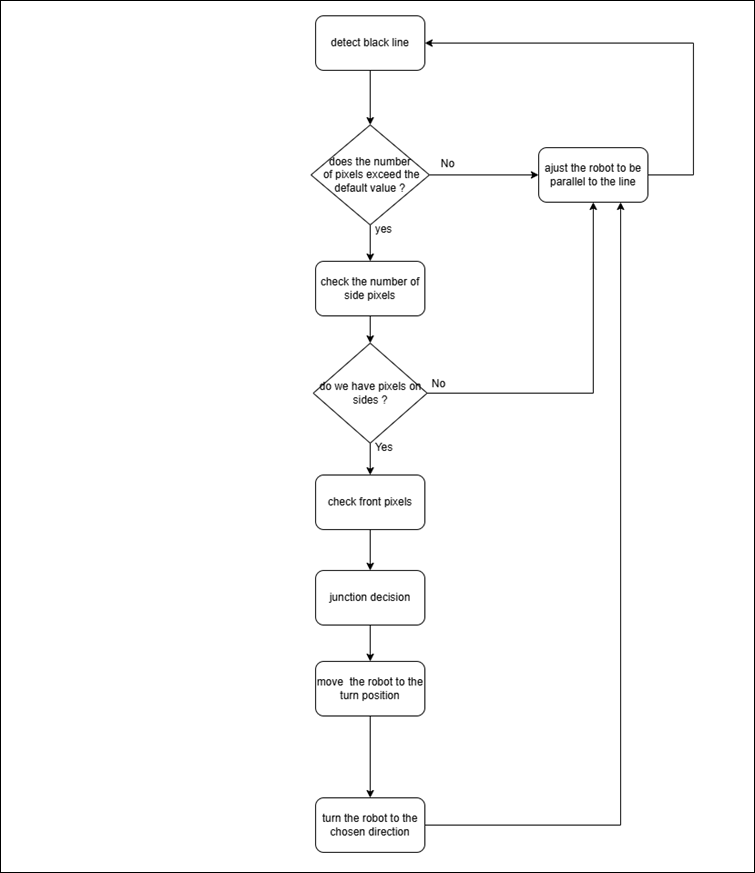
\includegraphics[width=\textwidth]{img/image043.png}
\caption{line following \& junction flowchart}
\label{judeFig31}
\end{figure}
\newpage
\paragraph{Example Scenario}

\begin{itemize}
\item
  \emph{Following a Straight Line: The robot detects a line with a small
  error and a number of black pixels within the threshold. The
  \_adjust\_orientation method adjusts the robot's orientation and moves
  it forward (see} \cref{judeFig30} Robot following the line and detecting a
  junction\emph{) .}
\item
  \emph{Approaching a Junction: The robot detects a significant increase
  in black pixels, indicating a junction.} The
  \emph{check\_side\_pixels} method detects more black pixels on the
  left side, suggesting a left turn. The \emph{check\_straight\_pixels}
  method confirms that the robot should stop and make a decision. The
  \emph{junction\_decision} method instructs the robot to turn left, so
  the robot move to the turn positrion (see \cref{judeFig31} the robot is at
  the turn position), and turn to the choosen direction (see \cref{judeFig32}
  The robot turns to the chosen direction).
\item
  Navigating a Complex Path: The robot uses a combination \emph{of
  check\_side\_pixels, check\_straight\_pixels,} and
  \emph{junction\_decision} to navigate through multiple junctions and
  reach its goal.
\end{itemize}


\begin{figure}[h!]
  \centering
  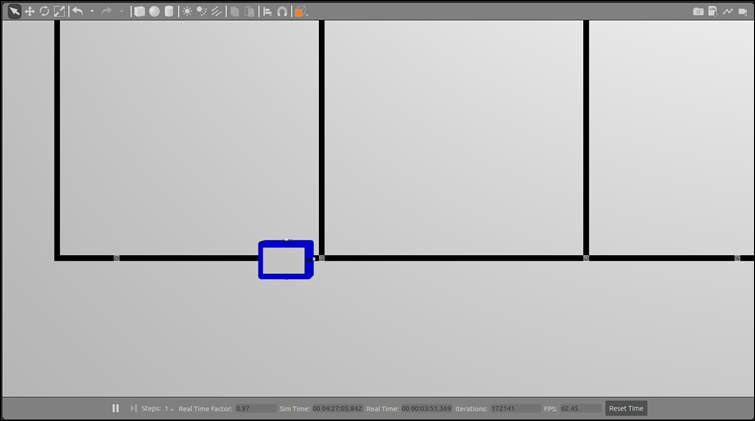
\includegraphics[width=\textwidth]{img/image045.png}
  \caption{Robot following the line and detecting a junction}
  \label{judeFig32}
  \end{figure}
\newpage
  \begin{figure}[h!]
    \centering
    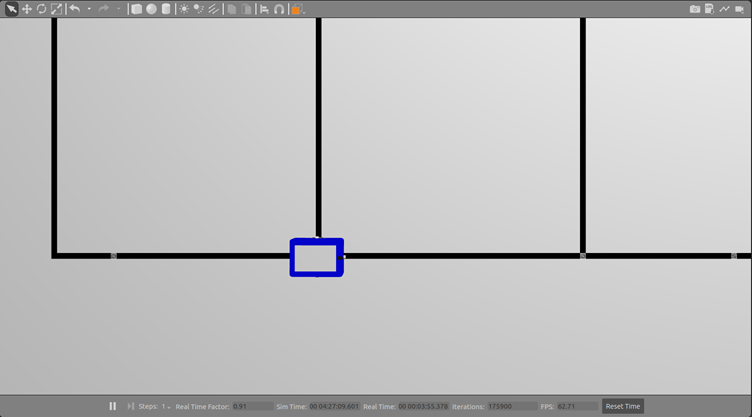
\includegraphics[width=\textwidth]{img/image047.png}
    \caption{the robot is at the turn position}
    \end{figure}

    \begin{figure}[h!]
      \centering
      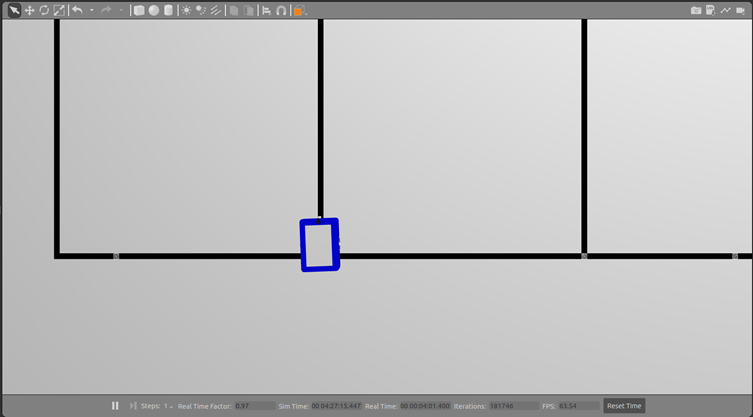
\includegraphics[width=\textwidth]{img/image049.png}
      \caption{The robot turns to the chosen direction}
      \end{figure}

\newpage

\paragraph{Essentials parameters}

The parameters (\emph{self.param, self.\_black\_pixels,
self.\_sideBlackPixels, self.\_threshold, self.\_middle\_width,
self.distanceToQr, and obstacle\_distance\_threshold}) are critical to
the functionality of the Task class. These values were carefully tuned
through \emph{extensive testing and experimentation} to ensure optimal
performance. Let's break down each parameter, its purpose, and how it
was determined:

\emph{\_black\_pixels:} Represents the expected number of black pixels
in the camera image when the robot is following a straight the line.
With a default Value of 493850, this value was determined by analyzing
the camera image when the robot is perfectly aligned on the line. This
parameter is used as a reference value for line-following logic. If the
number of black pixels deviates significantly from this value, the robot
adjusts its orientation.

\emph{\_sideBlackPixels:} Represents the expected number of black pixels
on the sides of the camera image when the robot is approaching a turn.
Its Value is 414556, Determined by analysing the camera image when the
robot is approaching a junction or turn.

It's used to detect when the robot should initiate a turn (e.g., when
the number of black pixels on one side exceeds this threshold).

\emph{\_threshold:} Defines the acceptable deviation from
self.\_black\_pixels for line-following.

The correct value found after test is 0.119 (11.9\%). This parameter
determined through experimentation to balance sensitivity and
robustness. If the number of black pixels deviates by more than 11.9\%
from self.\_black\_pixels, the robot adjusts its orientation.

\emph{\_middle\_width:} Defines the width of the region of interest
(ROI) in the camera image for line detection. Its value is 580 (pixels
width)\emph{.} Set to focus on the central portion of the camera image,
where the line is most likely to be.Adjusted to ensure the robot can
detect the line even if it deviates slightly from the center.

\emph{distanceToQr:} Represents the distance (in meters) from the robot
to the QR code when it is detected. With a value of 0.3869 meters,
determined by measuring the distance at which the QR code is reliably
detected and decoded and ensures the robot stops at an appropriate
distance from the QR code for accurate processing.

\emph{obstacle\_distance\_threshold}: Defines the minimum distance (in
meters) at which an obstacle is considered too close and requires
avoidance. Its value is 0.3 (meters).

Determined through testing to balance safety and efficiency. A smaller
value could risk collisions, while a larger value could cause
unnecessary detours.

\paragraph{How These Values Were Determined:}

\begin{itemize}
\item
  \emph{Iterative Testing}: Each parameter was initially set to a rough
  estimate based on theoretical calculations or prior experience. The
  robot was then tested in various scenarios (e.g., line following,
  obstacle avoidance, QR code detection) to observe its behaviour.
\item
  \emph{Incremental Adjustments}: Parameters were adjusted incrementally
  to improve performance. For example: Adjusting \emph{self.\_threshold}
  to reduce oscillations during line following.
\item
  \emph{Real-World Validation}: The robot was tested in real-world
  environments (e.g., with varying lighting conditions, uneven surfaces,
  and different obstacle configurations) to ensure robustness.
\item
  Trade-Offs: Some parameters required trade-offs. For example: A larger
  \emph{obstacle\_distance\_threshold} increases safety but may result
  in longer detours.
\end{itemize}

\paragraph{Child Classes: Mapping and Carrying}

The child classes (Mapping and Carrying) will extend the Task class to
implement task-specific logic.

\emph{Mapping}: Focuses on exploring the environment, detecting QR
codes, and building a map.

\emph{Carrying}: Focuses on transporting items between specified zones.

\subsubsection{Mapping}

The~\emph{Mapping class}~is designed to explore the environment, detect
QR codes, and store their positions in a database. It inherits from
the~\emph{Task class}, leveraging its core functionality such as robot
control, obstacle avoidance, and line following, while adding
mapping-specific logic to fulfill its unique role. This inheritance
allows the Mapping class to reuse existing methods and focus on
extending functionality for environment exploration and QR code
detection.

One of the key features of the Mapping class is~\emph{QR code
detection}, which is handled by the~\emph{\_check\_qr}~method. This
method detects QR codes using image processing techniques and stores the
detected QR codes along with their positions in a dictionary
(\emph{self.qrcodes}). To prevent duplicate detections, the class
compares new QR codes with the last detected one
(\emph{self.\_lastQrCode}), ensuring that each QR code is only recorded
once. This avoids redundancy and improves the efficiency of the mapping
process.

For~\emph{environment exploration}, the class utilizes
the~\emph{junction\_decision}~method to navigate junctions
systematically. When a junction is detected (e.g., left, right, or top),
the robot makes a decision to turn or move forward based on the
exploration strategy. This ensures that the robot explores all possible
paths in the environment, leaving no area unmapped. The systematic
approach guarantees comprehensive coverage, which is essential for
accurate mapping.

The Mapping class also integrates with an~\emph{SQLite
database}~(qr\_code.db) to store detected QR codes and their positions.
The~\emph{\_store~}method is responsible for inserting QR code data into
the database, while the~\emph{\_checkExistingQrCodes}~method checks for
existing QR codes to avoid redundant entries. This ensures that the
database remains up-to-date and free of duplicates. The database schema
includes a table named~\emph{qr\_code}~with columns for~id~(primary
key),~name~(QR code identifier),~position\_x~(X-coordinate),
and~position\_y~(Y-coordinate), providing a structured way to store and
retrieve mapping data.

When the mapping process is complete, the class emits a signal
(\emph{fsignal}) containing the detected QR codes, notifying other
system components of the task's completion. It also calls the parent
class's~\emph{\_task\_finished}~method to clean up resources and notify
the system, ensuring a smooth transition to the next task. The use of
the~\emph{signalslot} \emph{library}~enables decoupled communication
between the Mapping class and other components, enhancing modularity and
flexibility.

The class implements~\emph{robust error handling}~to manage potential
issues during database operations, such as table creation or data
insertion. Errors are logged using~\emph{rospy.logerr}, providing
detailed information for debugging and maintenance. Additionally, the
class ensures that the database connection is properly closed,
preventing resource leaks and ensuring data integrity.

\paragraph{How It Works}

The~\emph{Mapping class}~operates through a well-defined workflow that
ensures systematic environment exploration, QR code detection, and data
storage. Here's how it works in detail:

\emph{Initialization}

The Mapping class begins by initializing itself through the parent
class's constructor using~super().\_\_init\_\_("mapping"). This sets up
the core functionality inherited from the~\emph{Task class}, such as
robot control, obstacle avoidance, and line following. Additionally, the
class initializes the~\emph{fsignal}, a signal used to notify other
components when the mapping task is complete. This signal is essential
for decoupled communication within the system.

\emph{Start Mapping}

The mapping process is initiated by calling the~\emph{start}~method.
This method first checks for existing QR codes in the SQLite database
using the~\emph{\_checkExistingQrCodes}~method. If QR codes are already
present in the database, the task completes immediately by emitting
the~\emph{fsignal~}with the existing data. This avoids redundant mapping
and saves time. If no QR codes are found, the robot begins exploring the
environment, systematically navigating through the space to detect and
record new QR codes.

\emph{QR Code Detection}

QR code detection is handled by the~\emph{\_check\_qr}~method. When a QR
code is detected, the method processes it by converting its position to
global coordinates using the~\emph{\_calculate\_distance}~function. This
ensures that the QR code's location is accurately recorded relative to
the robot's environment. The detected QR code and its position are then
stored in the~\emph{self.qrcodes}~dictionary. To prevent duplicate
detections, the method compares the new QR code with the last detected
one (\emph{self.\_lastQrCode}). If the QR code has already been
recorded, it is ignored, ensuring that only unique QR codes are stored.

\begin{figure}
  \begin{minted}{js}
  def _check_qr(self, decoded_text):
    if not self._processQrCode :
      self._processQrCode = True
      if decoded_text[0] == "None" or decoded_text[0] is None:
          self._processQrCode = False
          return 
      if decoded_text[0] != self._lastQrCode:
          if len(self.qrcodes) >= 1:
            if (decoded_text[0] == list(self.qrcodes.keys())[0]):
                self._processQrCode = False
                self._task_finished(message="Mapping process finished")
                return     
          self.hasDetectedQrRecently = False
          position = self._calculate_distance(self.robot_pose)
          self.qrcodes[decoded_text[0]] = position
          self._lastQrCode = decoded_text[0]
          self._processQrCode = False
      self._processQrCode = False

\end{minted}
\caption{Mapping Qr Code Checker}
\end{figure}

\emph{Junction Navigation}

The~\emph{junction\_decision}~method plays a critical role in navigating
the robot through the environment. When the robot encounters a junction,
this method determines the appropriate action based on the type of
junction detected:

\begin{itemize}
\item
  If a~\emph{top junction}~is detected, the robot moves forward to
  continue exploration.
\item
  If a~\emph{left or right junction}~is detected, the robot prepares to
  turn, ensuring that all paths are systematically explored. This method
  ensures comprehensive coverage of the environment, leaving no area
  unmapped.
\end{itemize}

\begin{figure}
  \begin{minted}{python}
def junction_decision(self, onLeft, onRight, onTop):
    tm = 3
    if onTop:
    print("On top")
    tm = 1
    self._move_forward()
    self.timer= rospy.Timer(rospy.Duration(tm),self.resume_processing)
    elif onLeft:
        self._turnSide = "left"
        self.moveToTurnPosition = True
    elif onRight:
        self._turnSide = "right"
        self.moveToTurnPosition = True

\end{minted}
\caption{Junction decision of mapping class}
\end{figure}

\emph{Task Completion}

Once the mapping process is complete, the~\emph{\_task\_finished}~method
is called to wrap up the task. This method performs several key actions:

\begin{enumerate}
\def\labelenumi{\arabic{enumi}.}
\item
  It stores the detected QR codes in the SQLite database using
  the~\emph{\_store}~method, ensuring that the data is saved for future
  use.
\item
  It emits the~\emph{fsignal}~with the QR code data, notifying other
  system components that the task is complete.
\item
  It calls the parent class's~\emph{\_task\_finished}~method to clean up
  resources and notify the system, ensuring a smooth transition to the
  next task.
\end{enumerate}

\paragraph{Impact on the System}

The Mapping class enables the robot to \emph{autonomously explore its
environment}, \emph{detect QR codes}, and \emph{store their positions}
for future use. It leverages the parent class's functionality for robot
control and obstacle avoidance, demonstrating the power of
\emph{inheritance} and \emph{code reuse}. The integration with SQLite
ensures \emph{persistent storage} of mapping data, enabling other tasks
(e.g., carrying) to use this information.

\subsubsection{Carrying}

The~\emph{Carrying class}~is a specialized child class of the~\emph{Task
class}, designed to handle the transportation of items between specified
zones. It extends the parent class by adding carrying-specific
functionality, such as QR code navigation, lifting mechanism control,
and complex junction navigation. By leveraging the core functionality of
the Task class---such as robot control, obstacle avoidance, and line
following---the Carrying class focuses on implementing logic tailored to
item transportation tasks.

\paragraph{Key Features and Functionality}

\emph{Task Initialization:}\\
The Carrying class initializes by accepting a list of tasks (params)
that specify the zones and actions to be performed, such as loading or
unloading. It calls the parent class's constructor with the task
name~"carrying"~to set up the core functionality. This initialization
ensures the robot is ready to execute the carrying task with the
necessary parameters.

\emph{QR Code Navigation:}\\
The class uses QR codes to navigate to goal positions. It implements
the~\emph{\_check\_qr}~method to detect QR codes and determine if the
robot has reached a goal zone. By comparing the detected QR code with
the target zone, the robot can confirm its location and proceed with the
next action, such as loading or unloading.

\emph{Lifting Mechanism:}\\
The Carrying class controls a lifting mechanism to handle items during
loading and unloading. The~\emph{\_lift}~method is responsible for
interpolating the lifting motion over a specified duration, ensuring
smooth and precise movement. Commands for the lifting mechanism are
published to the~\emph{/position\_joint\_controller/command}~topic,
enabling real-time control.

\emph{Junction Navigation:}\\
The class extends the~\emph{junction\_decision}~method to handle complex
navigation decisions. When the robot encounters a junction, it
determines the best direction to reach the goal zone based on QR code
positions and intersections. The class uses a~\emph{shortest path
algorithm}~to choose between turning left, right, or making a U-turn,
ensuring efficient navigation.

\emph{Task Completion:}\\
The class tracks the progress of the task
using~\emph{self.\_currentTask}. Once all goals have been reached, the
task is marked as complete, and a signal (\emph{fsignal}) is emitted to
notify the system. This ensures that other components are aware of the
task's completion and can take appropriate action.

\paragraph{How It Works}
\emph{Initialization:}\\
The Carrying class initializes by calling the parent class's constructor
and setting up the task parameters. It prepares the robot for the
carrying task by loading QR code positions and configuring the lifting
mechanism.

\emph{Navigation and QR Code Detection.}\\
The robot navigates through the environment using QR codes as markers.
The~\emph{\_check\_qr}~method detects QR codes and determines if the
robot has reached a goal zone. If the target zone is reached, the robot
proceeds with loading or unloading.

\emph{Lifting Mechanism Control:}\\
The~\emph{\_lift}~method controls the lifting mechanism, interpolating
its motion to ensure smooth operation. This method is called during
loading and unloading to handle items efficiently.

\emph{Junction Navigation:}\\
The~\emph{junction navigation} is a critical component of the Carrying
class, responsible for handling navigation decisions at junctions. Its
purpose is to determine the best action---such as turning left, right,
or moving forward---based on the detected QR codes, the robot's current
position, and the goal zone. This method ensures the robot navigates
efficiently and reaches its destination while avoiding unnecessary
detours.

The method takes three key parameters: \emph{onLeft} Indicates whether a
left turn is detected, \emph{onRight} Indicates whether a right turn is
detected and \emph{onTop} Indicates whether a straight path is detected.
These parameters provide information about the robot's immediate
environment, helping it decide the best course of action.

The method's logic is divided into two main scenarios: when no QR code
is detected and when a QR code is detected.

\emph{No QR Code Detected:} If no QR code has been scanned recently, the
robot makes a decision based on the detected junctions:

\begin{itemize}
\item
  If a~\emph{left or right turn}~is detected, the robot prepares to turn
  in the corresponding direction.
\item
  If a~\emph{straight path}~is detected, the robot moves forward to
  continue its journey.
\end{itemize}

This logic ensures the robot continues exploring or navigating even when
no QR codes are present, maintaining progress toward its goal.

\emph{QR Code Detected:} If a QR code has been scanned, the robot checks
whether it corresponds to a~\emph{goal zone}~or an~\emph{intersection}:

\begin{itemize}
\item
  If the QR code is a~\emph{goal zone}, the robot moves to the lifting
  position and performs the required action, such as loading or
  unloading. This marks a key milestone in the task.
\item
  If the QR code is an~\emph{intersection}, the robot uses
  the~\emph{\_chooseSide~}or~\emph{\_chooseSideToGo}~method to determine
  the best direction to reach the goal zone. These methods calculate the
  optimal path based on the robot's current position, the goal zone's
  location, and the available routes.
\end{itemize}

This logic ensures the robot makes informed decisions at intersections,
minimizing travel time and energy consumption.

Based on the decision-making process, the method publishes velocity
commands (self.msg) to the~\emph{/cmd\_vel}~topic. These commands
execute the chosen action, such as turning left, turning right, or
moving forward. This ensures the robot's movements are precise and
aligned with the navigation strategy.


\begin{minted}{python}
def junction_decision(self, onLeft, onRight, onTop):
    print("Making decision")
    print(self.hasDetectedQrRecently)
    self.stop()
    tm = 3
    current = self._params[self._currentTask]
        
    if not self.hasDetectedQrRecently:  # no qrCode has been scanned
        if onLeft and (not onTop) and (not onRight): 
            self._turnSide = "left"
            self.moveToTurnPosition = True
        elif onRight and (not onTop) and (not onLeft): 
            self._turnSide = "right"
            self.moveToTurnPosition = True
        elif onTop: 
            tm = 2
            self._move_forward()        
            self.timer = rospy.Timer(rospy.Duration(tm), self.resume_processing, oneshot=True)
        else:  # if the robot can't go straight, failed the task
            self._task_failed("The robot is stuck : should go straight")
   
    elif self._lastQrCode:  # qrCode has been scanned
        if self._lastQrCode in self.qrcodes:  
            if self._isStationSide(self._lastQrCode):
                tm = 2
                self._move_forward()        
                self.timer = rospy.Timer(rospy.Duration(tm), self.resume_processing, oneshot=True)
            else:
                if self.goal_in_db:
                    current = self._params[self._currentTask]
                    zArr = current["zone"].split(" ")
                    goal = f"{zArr[0]}_{zArr[1]}_center"
                    goalPos = self.qrcodes.get(goal, (None, None))
                    side = self._chooseSideToGo(onTop, onRight, onLeft, goalPos)
                    if side == "S":
                        tm = 2
                        self._move_forward()        
                        self.timer = rospy.Timer(rospy.Duration(tm), self.resume_processing, oneshot=True)
                    elif side == "R":
                        self._turnSide = "right"
                        self.moveToTurnPosition = True
                    elif side == "L":
                        self._turnSide = "left"
                        self.moveToTurnPosition = True
                    elif side == "B":
                        tm = 6
                        self._U_turn()         
                        self.timer = rospy.Timer(rospy.Duration(tm), self.resume_processing, oneshot=True)
                    elif side == "0":
                        return
                else:  
                    intersections = self._getIntersection(current['zone']) 
                    if self._lastQrCode in [intersections[0][0], intersections[1][0]]: 
                        if onLeft:                  
                            self._turnSide = "left"
                            self.moveToTurnPosition = True
                        elif onRight:
                            self._turnSide = "right"
                            self.moveToTurnPosition = True
                        else: 
                            self._task_failed("The robot is stuck : should turn") 
                    else: 
                        if onLeft and (not onTop) and (not onRight):
                            self._turnSide = "left"
                            self.moveToTurnPosition = True
                        elif onRight and (not onTop) and (not onLeft): 
                            self._turnSide = "right"
                            self.moveToTurnPosition = True
                        else: 
                            print("Not a corner, using shortest path")
                            side = self._chooseSide(onTop, onRight, onLeft, intersections)
                            if side == "S":
                                tm = 2
                                self._move_forward()        
                                self.timer = rospy.Timer(rospy.Duration(tm), self.resume_processing, oneshot=True)
                            elif side == "R":
                                self._turnSide = "right"
                                self.moveToTurnPosition = True
                            elif side == "L":
                                self._turnSide = "left"
                                self.moveToTurnPosition = True
                            elif side == "B":
                                tm = 6
                                self._U_turn()         
                                self.timer = rospy.Timer(rospy.Duration(tm), self.resume_processing, oneshot=True)
                            elif side == "0":
                                tm = 6
                                self._U_turn()         
                                self.timer = rospy.Timer(rospy.Duration(tm), self.resume_processing, oneshot=True)
                                rospy.logerr("Wrong direction")
                                return
        else:
            tm = 2
            self._move_forward()        
            self.timer = rospy.Timer(rospy.Duration(tm), self.resume_processing, oneshot=True)
            rospy.logerr("The robot is stuck : doesn't know what to do")
\end{minted}
% \caption{Junction Decision Function Of Carrying Process}
\captionof{figure}{Junction Decision Function Of Carrying Process}\label{judeFig37}

\emph{Task Completion:}
Once all goals have been reached, the task is marked as complete, and
the~\emph{fsignal}~is emitted to notify the system. The parent class's
cleanup methods are called to ensure resources are released and the
system is ready for the next task.

\paragraph{Interaction Between Methods}

\begin{itemize}
\item
  \emph{Junction Detection}: The junction\_decision method detects
  junctions and determines if the robot should turn left, right, or move
  forward. If a QR code is detected, it uses \_chooseSide or
  \_chooseSideToGo to determine the best direction to reach the goal
  zone.
\item
  \emph{Path Planning}: The \_chooseSide method calculates the shortest
  path to the goal zone based on the positions of intersections. The
  \_chooseSideToGo method calculates the shortest path to a specific
  target position (e.g., a goal zone).
\item
  \emph{Navigation}:

  \begin{itemize}
  \item
    Based on the chosen direction, the robot executes the corresponding
    action (e.g., turn left, turn right, move forward).
  \end{itemize}
\end{itemize}

\paragraph{Example Scenario}

\begin{enumerate}
\def\labelenumi{\arabic{enumi}.}
\item
  Approaching a Junction: The robot detects a junction with options to
  turn left, right, or move forward. The \emph{junction\_decision}
  method calls \emph{\_chooseSide} to determine the best direction to
  reach the goal zone.
\item
  Calculating the Shortest Path: The \emph{\_chooseSide} method
  calculates the Euclidean distance to each intersection and chooses the
  direction with the minimum distance. If the goal zone is directly
  ahead, the robot moves forward. If it's to the left or right, the
  robot turns accordingly.
\item
  Executing the Action: The robot executes the chosen action (e.g., turn
  left, turn right, move forward) and continues navigating toward the
  goal zone.
\end{enumerate}
\newpage
\paragraph{Impact on the System}

\begin{itemize}
\item
  These methods enable the robot to \emph{autonomously navigate
  junctions} and \emph{reach goal zones efficiently}, ensuring reliable
  and efficient task execution.
\item
  They demonstrate the importance of \emph{path planning} and
  \emph{decision-making algorithms} in robotics, showcasing your ability
  to implement complex navigation logic.
\end{itemize}

\begin{figure}
  \begin{minted}{python}
def _adjust_orientation(self, error, angle, pixels, mask, w_min, h_min):
        
        if not self.isLifting :
            if self.moveToLiftPosition:
                if self._distanceToLifePosition() > 0.005:
                    self._move(error)
                    return None
                else:
                    print("Lift position reached")
                    self.stop()
                    self.isLifting = True
                    self._lift()
                return None
            else:
                return super()._adjust_orientation(error, angle, pixels, mask, w_min, h_min)

\end{minted}
\caption{Adjust Orientation Function of Carrying Class}
\end{figure}

\begin{figure}[h!]
  \begin{minted}{python}
def _lift(self, duration=3):
    current = self._params[self._currentTask]
    liftType = current["type"]
    start = 0 if liftType == "Loading" else 1
    end = 1 if liftType == "Loading" else 0

    start_time = rospy.Time.now()
    end_time = start_time + rospy.Duration.from_sec(duration)
    rate = rospy.Rate(100)  
    while rospy.Time.now() < end_time and not rospy.is_shutdown():
        current_time = rospy.Time.now()
        elapsed = (current_time - start_time).to_sec()
        fraction = elapsed / duration
        fraction = min(fraction, 1.0)  # Fixed the missing parenthesis here
        current_value = start + fraction * (end - start)
        self.liftPub.publish(current_value)
        rate.sleep()

    self.liftPub.publish(end)
    self.isLifting = False
    self.moveToLiftPosition = False

    self._currentTask += 1
    if(self._currentTask == len(self._params)):
        self.stop()
        self._task_finished(message="All goals have been reached")
\end{minted}
\caption{Lift function}
\end{figure}

\begin{figure}[h!]
\centering
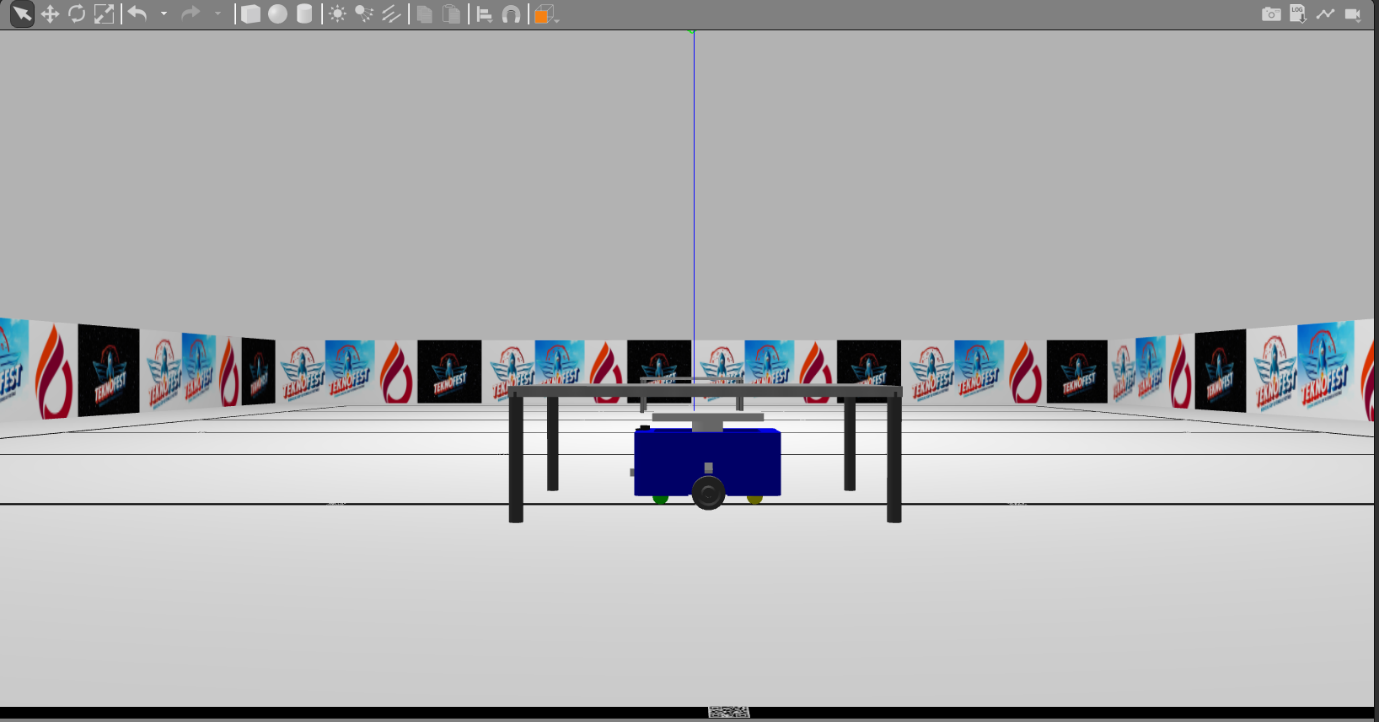
\includegraphics[width=\textwidth]{img/image057.png}
\caption{the robot ready to lift a charge}
\end{figure}




\end{document}